%%% Supporting_information.Rnw --- 

%% Author: emanuelheitlinger@gmail.com

\documentclass[12pt,a4paper]{article}
\usepackage[debugshow,final]{graphics}
\usepackage{hyperref}
\usepackage{float}
\usepackage{lscape} 
\usepackage{rotating} 
 

\date{}
\usepackage{/home/ele/tools/R-devel/share/texmf/tex/latex/Sweave}
\begin{document}

\title{Addtional figures, tables and text describing the assembly
  process for ``The transcriptome of the invasive eel swimbladder
  nematode parasite \textit{Anguillicola crassus}'' (Heitlinger et
  al.)}

\maketitle
\tableofcontents
\listoffigures 
\listoftables

% make the plots modest size

\renewcommand{\figurename}{Additional Figure}
\renewcommand{\tablename}{Additional Table}

\section{Additional figures referenced in the main text}

\newpage
\clearpage

\begin{sidewaysfigure}
  \centering
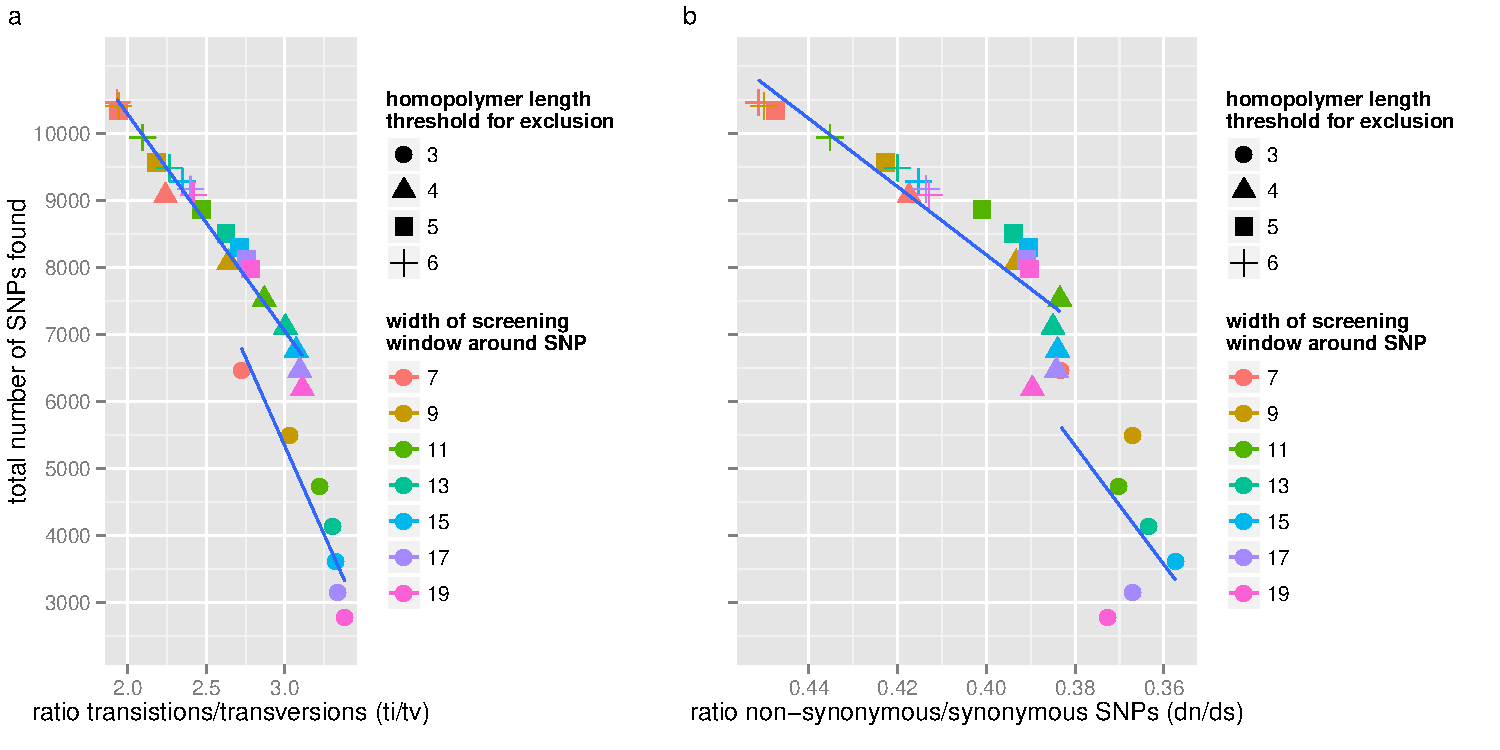
\includegraphics{../figures/Additional_Figure_1.pdf}
\caption[Filtering of putative SNPs]{Filtering of putative SNPs. When
  SNPs in or adjacent to homopolymeric regions are removed changes in
  ti/tv and dn/ds are observed: as the overall number of SNPs is
  reduced both ratios change to more plausible values. Note the
  reversed axis for dn/ds to plot these lower values to the right. For
  homopolymer length $>$ 3 a linear trend for the total number of SNPs
  and the two measurements is observed. A width of 11 for the
  screening window provides most plausible values (suggesting
  specificity) while still incorporating a high number of SNPs
  (sensitivity).}
\end{sidewaysfigure}

\newpage
\clearpage

\begin{sidewaysfigure}
  \centering
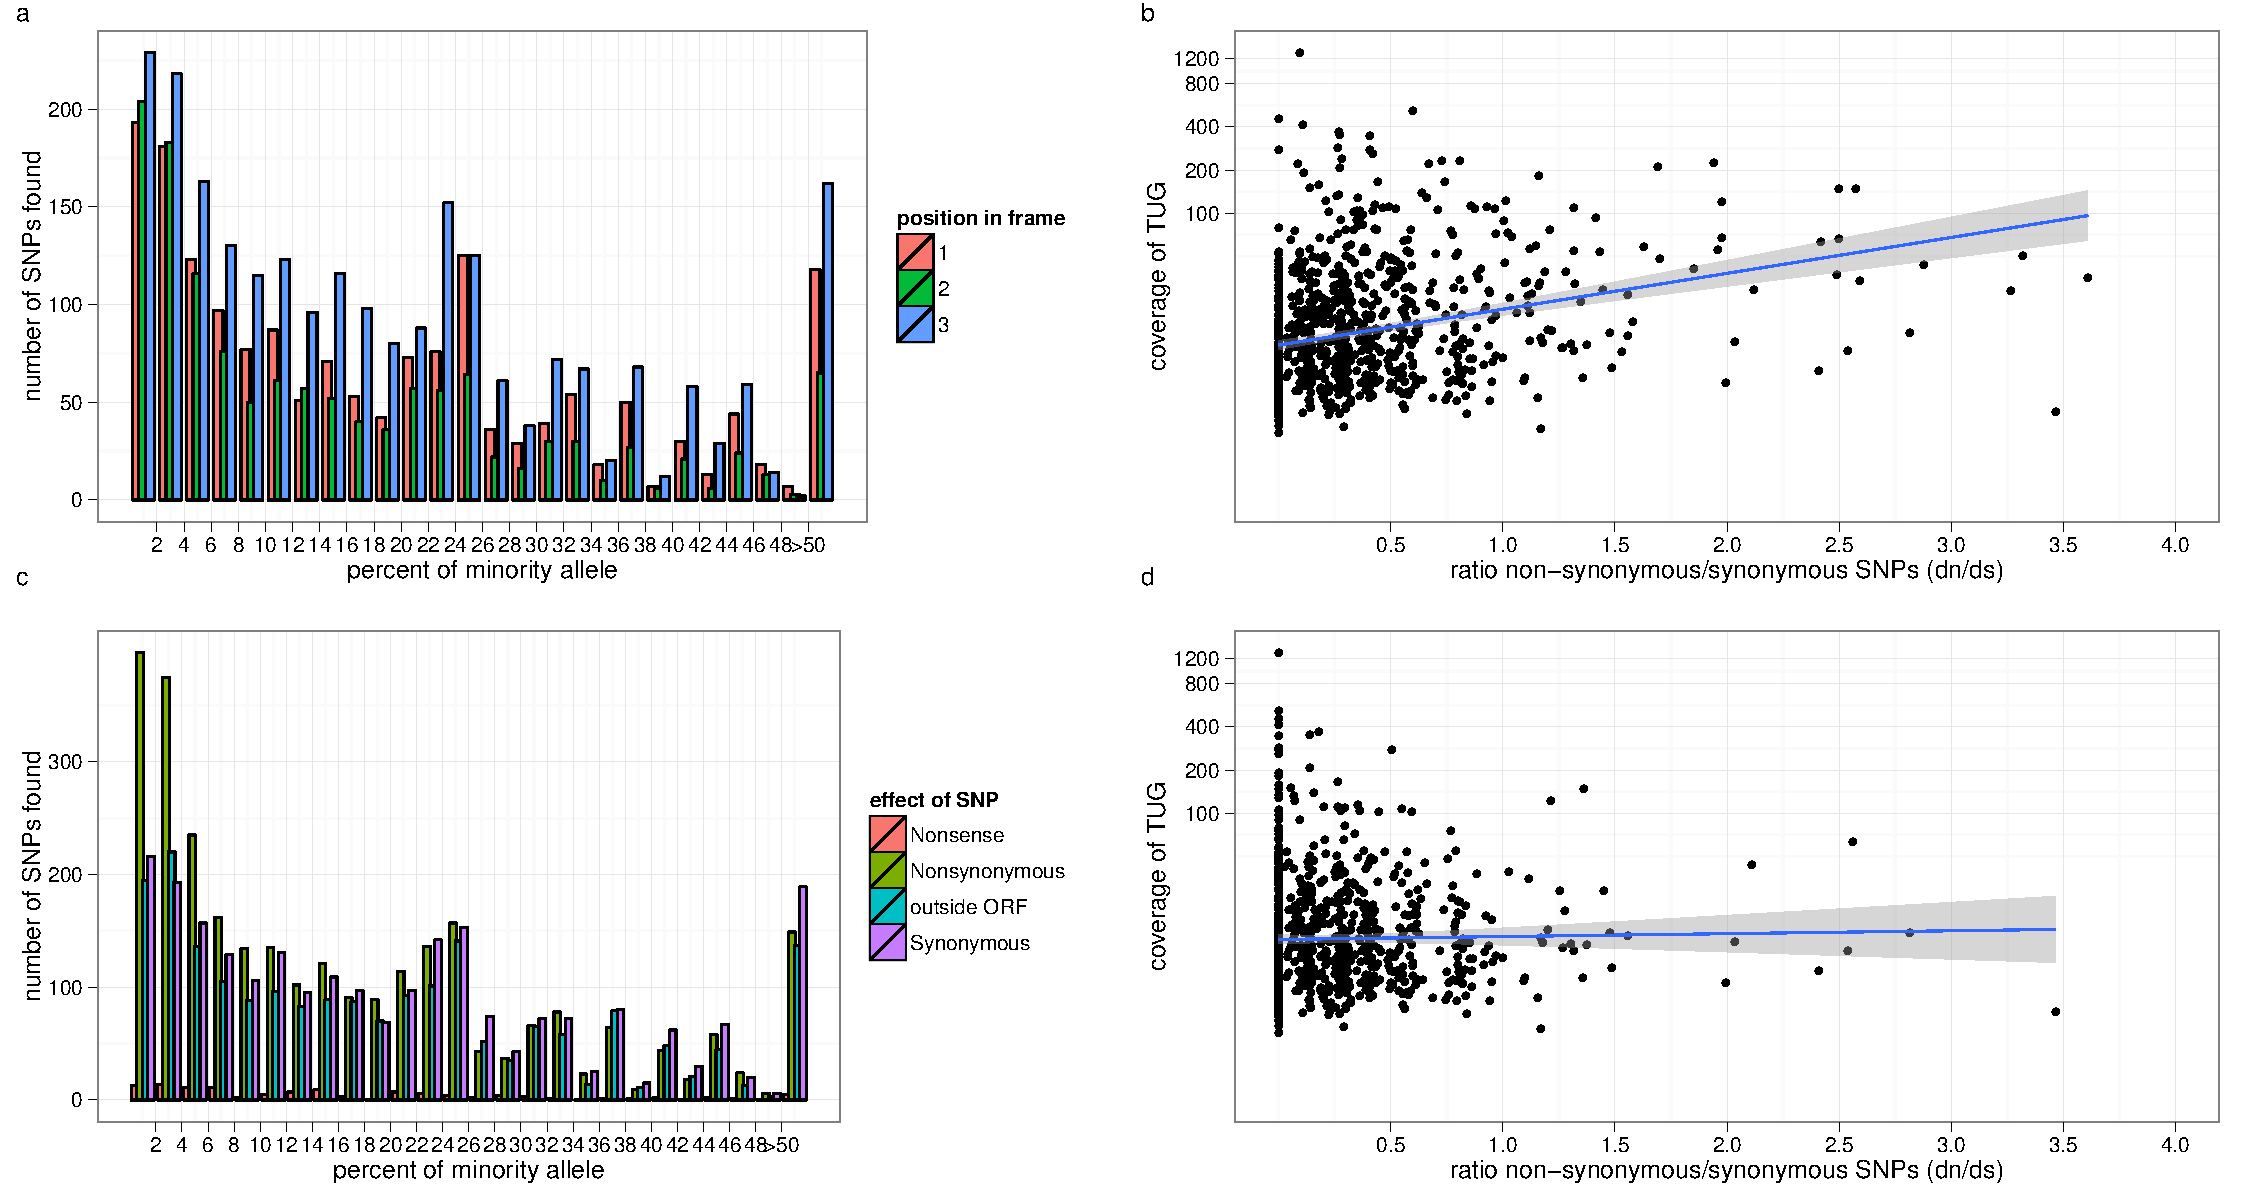
\includegraphics{../figures/Additional_Figure_2.pdf}
\caption[SNP distribution is affected by codon position and
coverage]{SNP distribution is affected by codon position and
  coverage. Overabundance of SNPs at codon-position two (a) and of
  non-synonymous SNPs (c) for low percentages of the minority
  allele. (b) Significant positive correlation of coverage and dn/ds
  before removing these SNPs at a threshold of 7\% ($p<$ 0.001, $R^2=$
  0.015) and (d) absence of such a correlation afterwards ($p=$0.192,
  $R^2<$0.001).}
\end{sidewaysfigure}

\newpage
\clearpage

\begin{sidewaysfigure}
  \centering
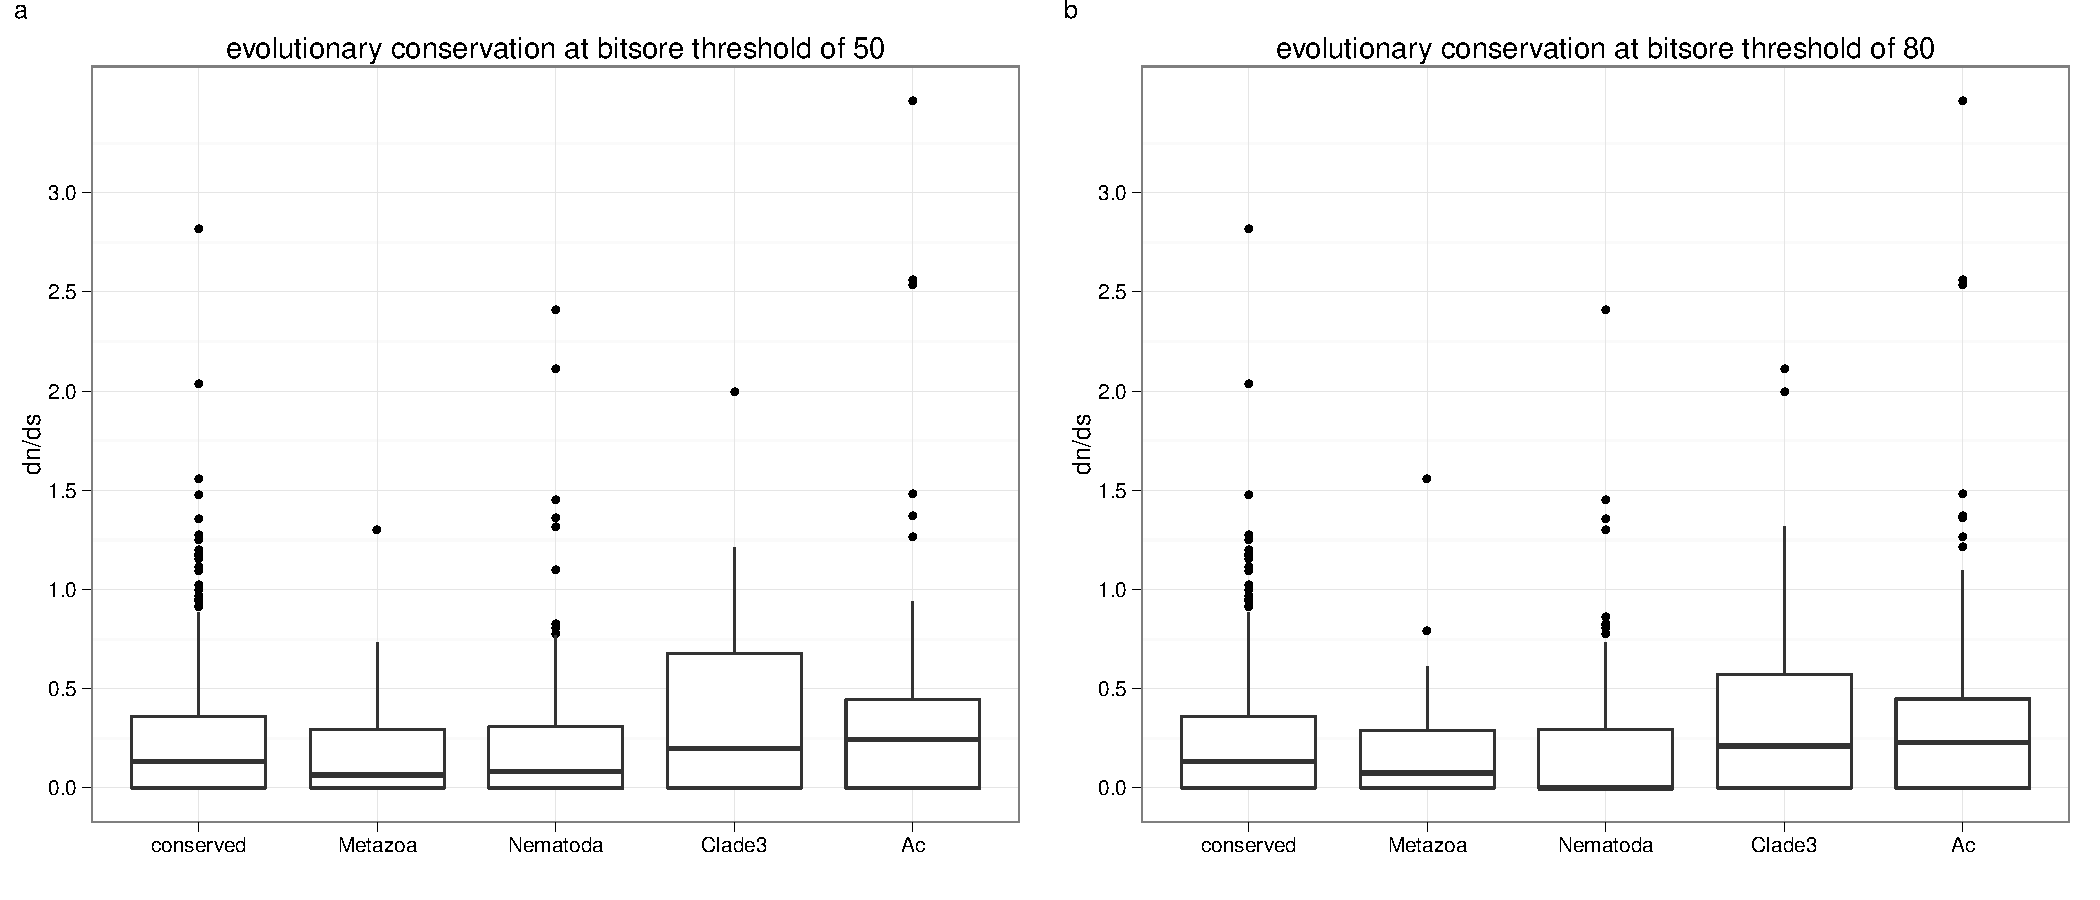
\includegraphics{../figures/Additional_Figure_3.pdf}
\caption[Positive selection by categories of evolutionary
conservation]{Positive selection by categories of evolutionary
  conservation. Boxplot of dn/ds based on the screened set of SNPs in
  TUGs by different categories of evolutionary
  conservation. Significant comparisons are sequences novel in Metazoa
  vs. novel in \textit{A. crassus} (0.009 and 0.002; p-value for
  bitscore of 50 and 80, Nemenyi-Damico-Wolfe-Dunn test), in Nematoda
  vs. in \textit{A. crassus} (0.03 and 0.009). Sequences novel in
  Spirurina failed to show significantly elevated dn/ds, despite
  higher median values due to the low number of contigs of this
  category with a dn/ds obtained.}
\end{sidewaysfigure}

\newpage
\clearpage

% \begin{sidewaysfigure}
%   \centering
%   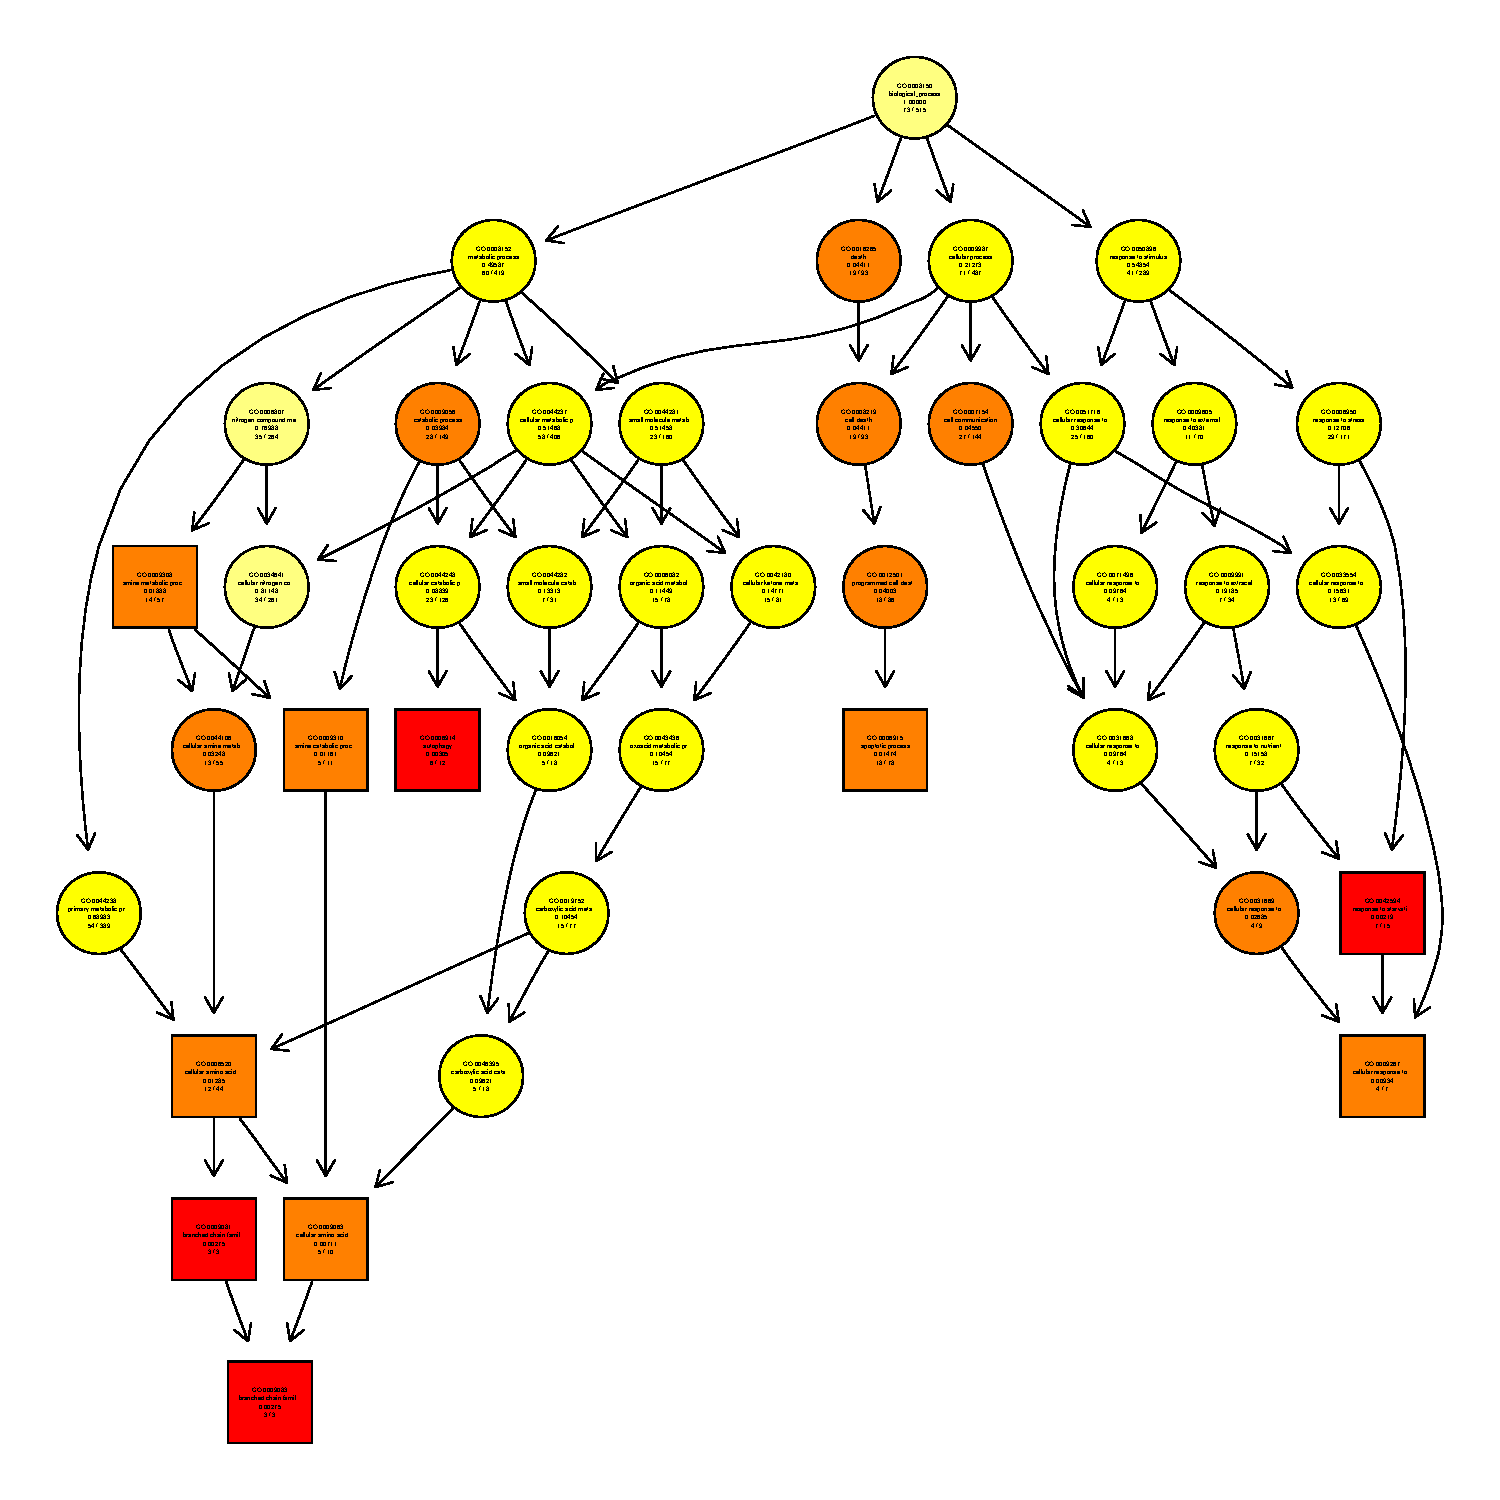
\includegraphics[width=23cm]{../figures/tGO_DN_DS_BP_classic_10_all}
%   \caption[GO biological process graph for enriched terms in contigs
%   under positive selection]{GO biological process graph for enriched
%     terms in contigs under positive selection. Subgraph of the
%     GO-ontology biological process category induced by the top 10
%     terms identified as enriched contigs under positive
%     selection. Boxes indicate the 10 most significant terms. Box
%     colour represents the relative significance, ranging from dark red
%     (most significant) to light yellow (least significant). In each
%     node the category-identifier, a (eventually truncated) description
%     of the term, the significance for enrichment and the number of DE
%     / total number of annotated genes is given. Black arrows indicate
%     an ``is-a'' relationship.}{1.3}
% \end{sidewaysfigure}

% \newpage
% \clearpage

% \begin{sidewaysfigure}
%   \centering
%   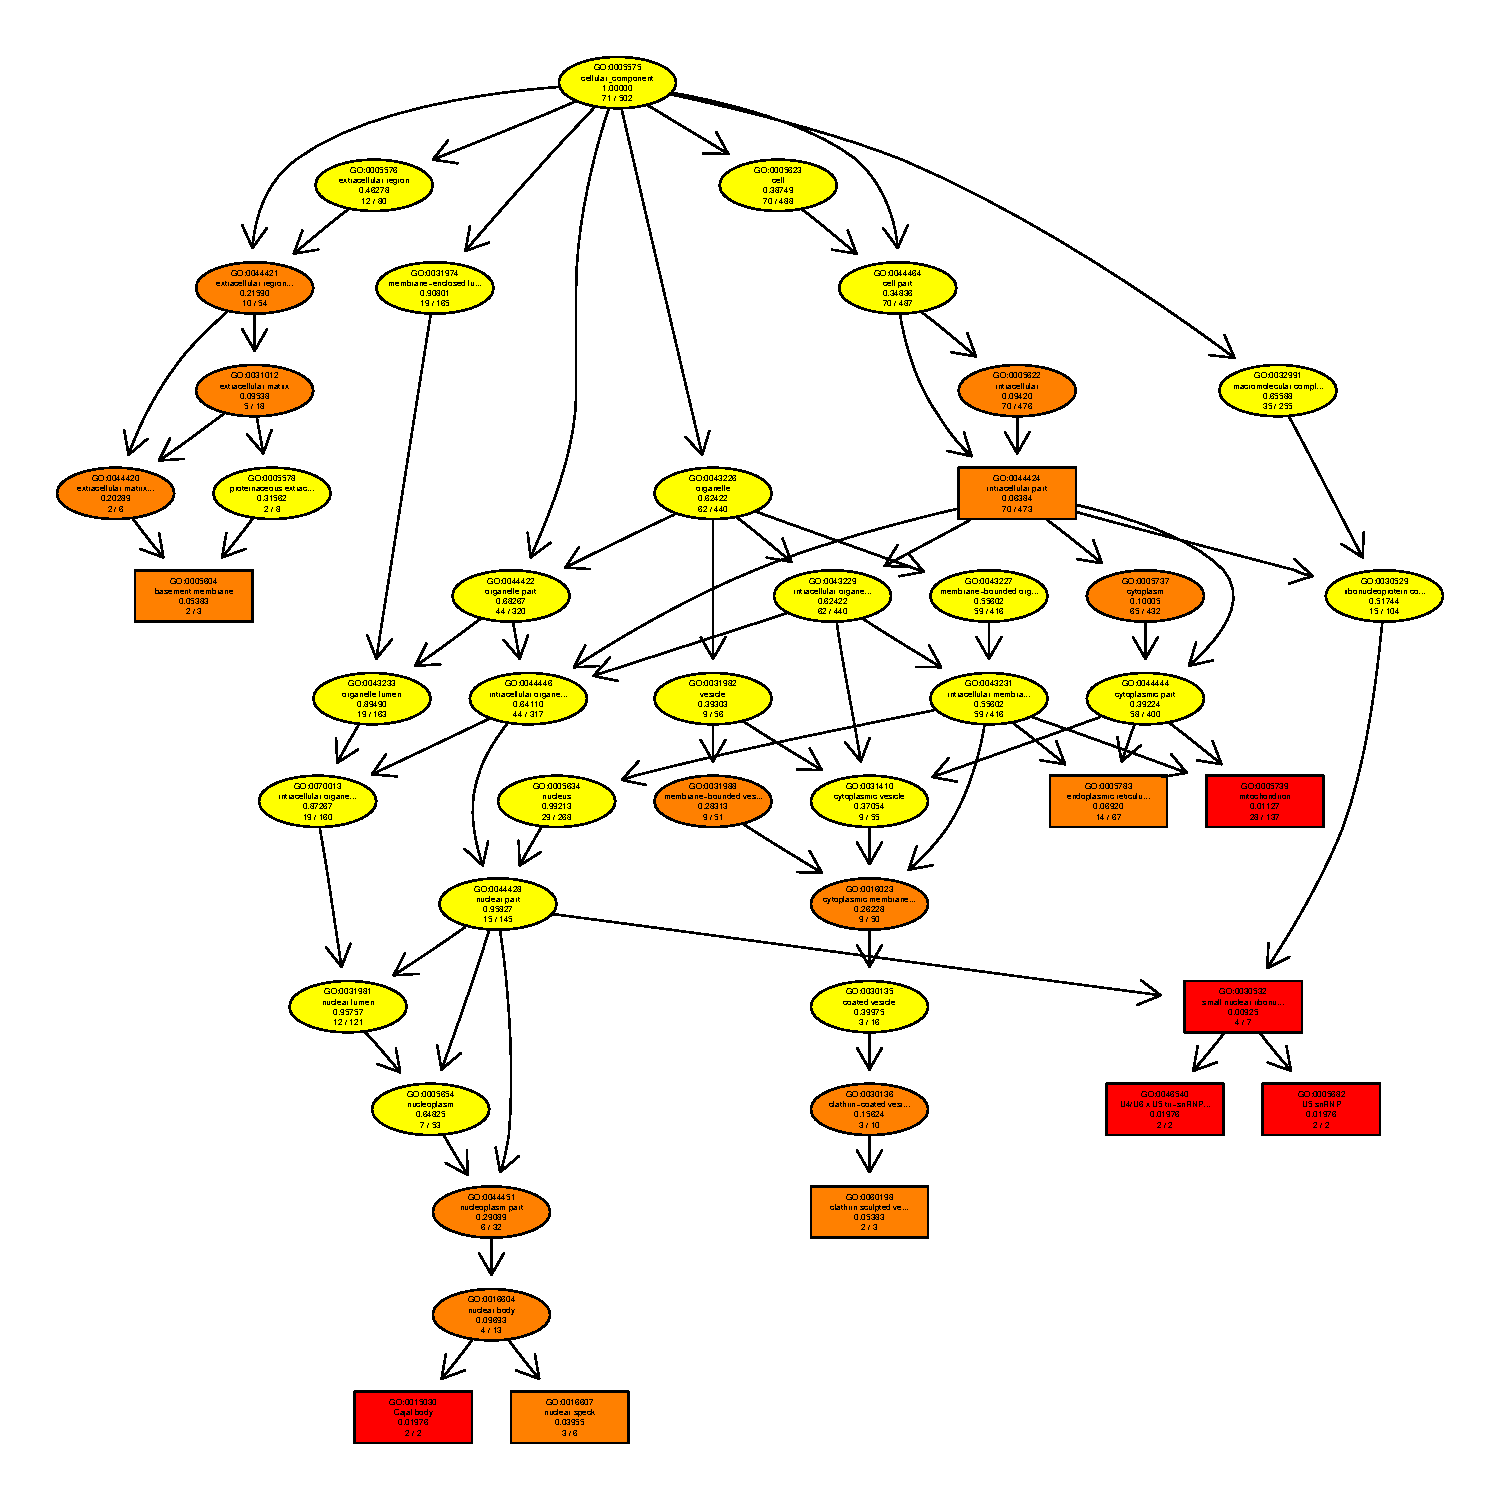
\includegraphics{../figures/tGO_DN_DS_CC_classic_10_all}
%   \caption[GO cellular compartment graph for enriched terms in contigs
%   under positive selection]{GO cellular compartment graph for enriched
%     terms in contigs under positive selection. Subgraph of the
%     GO-ontology cellular compartment category induced by the top 10
%     terms identified as enriched contigs under positive
%     selection. Boxes indicate the 10 most significant terms. Box
%     colour represents the relative significance, ranging from dark red
%     (most significant) to light yellow (least significant). In each
%     node the category-identifier, a (eventually truncated) description
%     of the term, the significance for enrichment and the number of DE
%     / total number of annotated genes is given. Black arrows indicate
%     an ``is-a'' relationship.}{1.3}
% \end{sidewaysfigure}

% \newpage
% \clearpage

% \begin{sidewaysfigure}
%   \centering
%   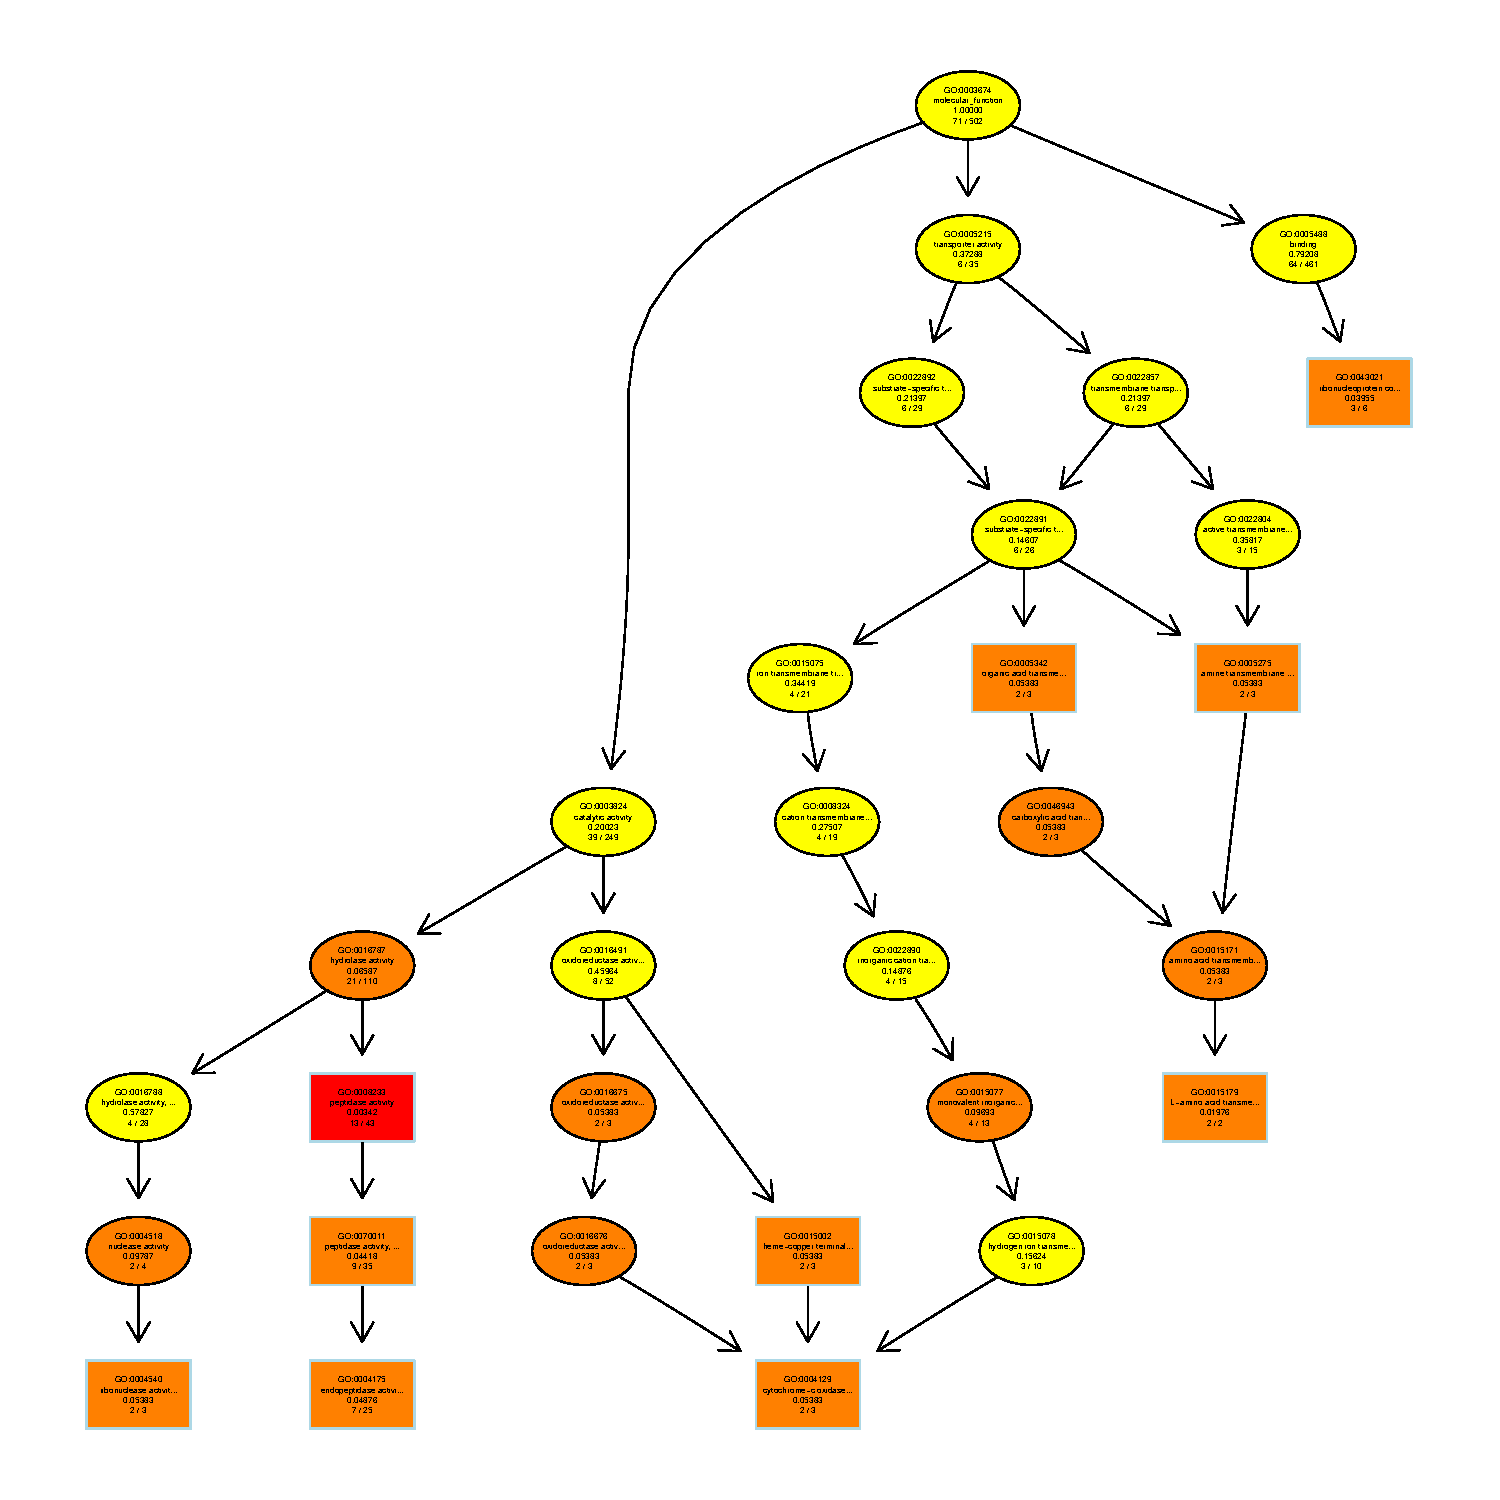
\includegraphics{../figures/tGO_DN_DS_MF_classic_10_all}
%   \caption[GO molecular function graph for enriched terms in contigs
%   under positive selection]{GO molecular function graph for enriched
%     terms in contigs under positive selection. Subgraph of the
%     GO-ontology biological process category induced by the top 10
%     terms identified as enriched contigs under positive
%     selection. Boxes indicate the 10 most significant terms. Box
%     colour represents the relative significance, ranging from dark red
%     (most significant) to light yellow (least significant). In each
%     node the category-identifier, a (eventually truncated) description
%     of the term, the significance for enrichment and the number of DE
%     / total number of annotated gene is given. Black arrows indicate
%     an ``is-a'' relationship.}{1.3}
% \end{sidewaysfigure}

% \newpage
% \clearpage

% \begin{sidewaysfigure}
%   \centering
%   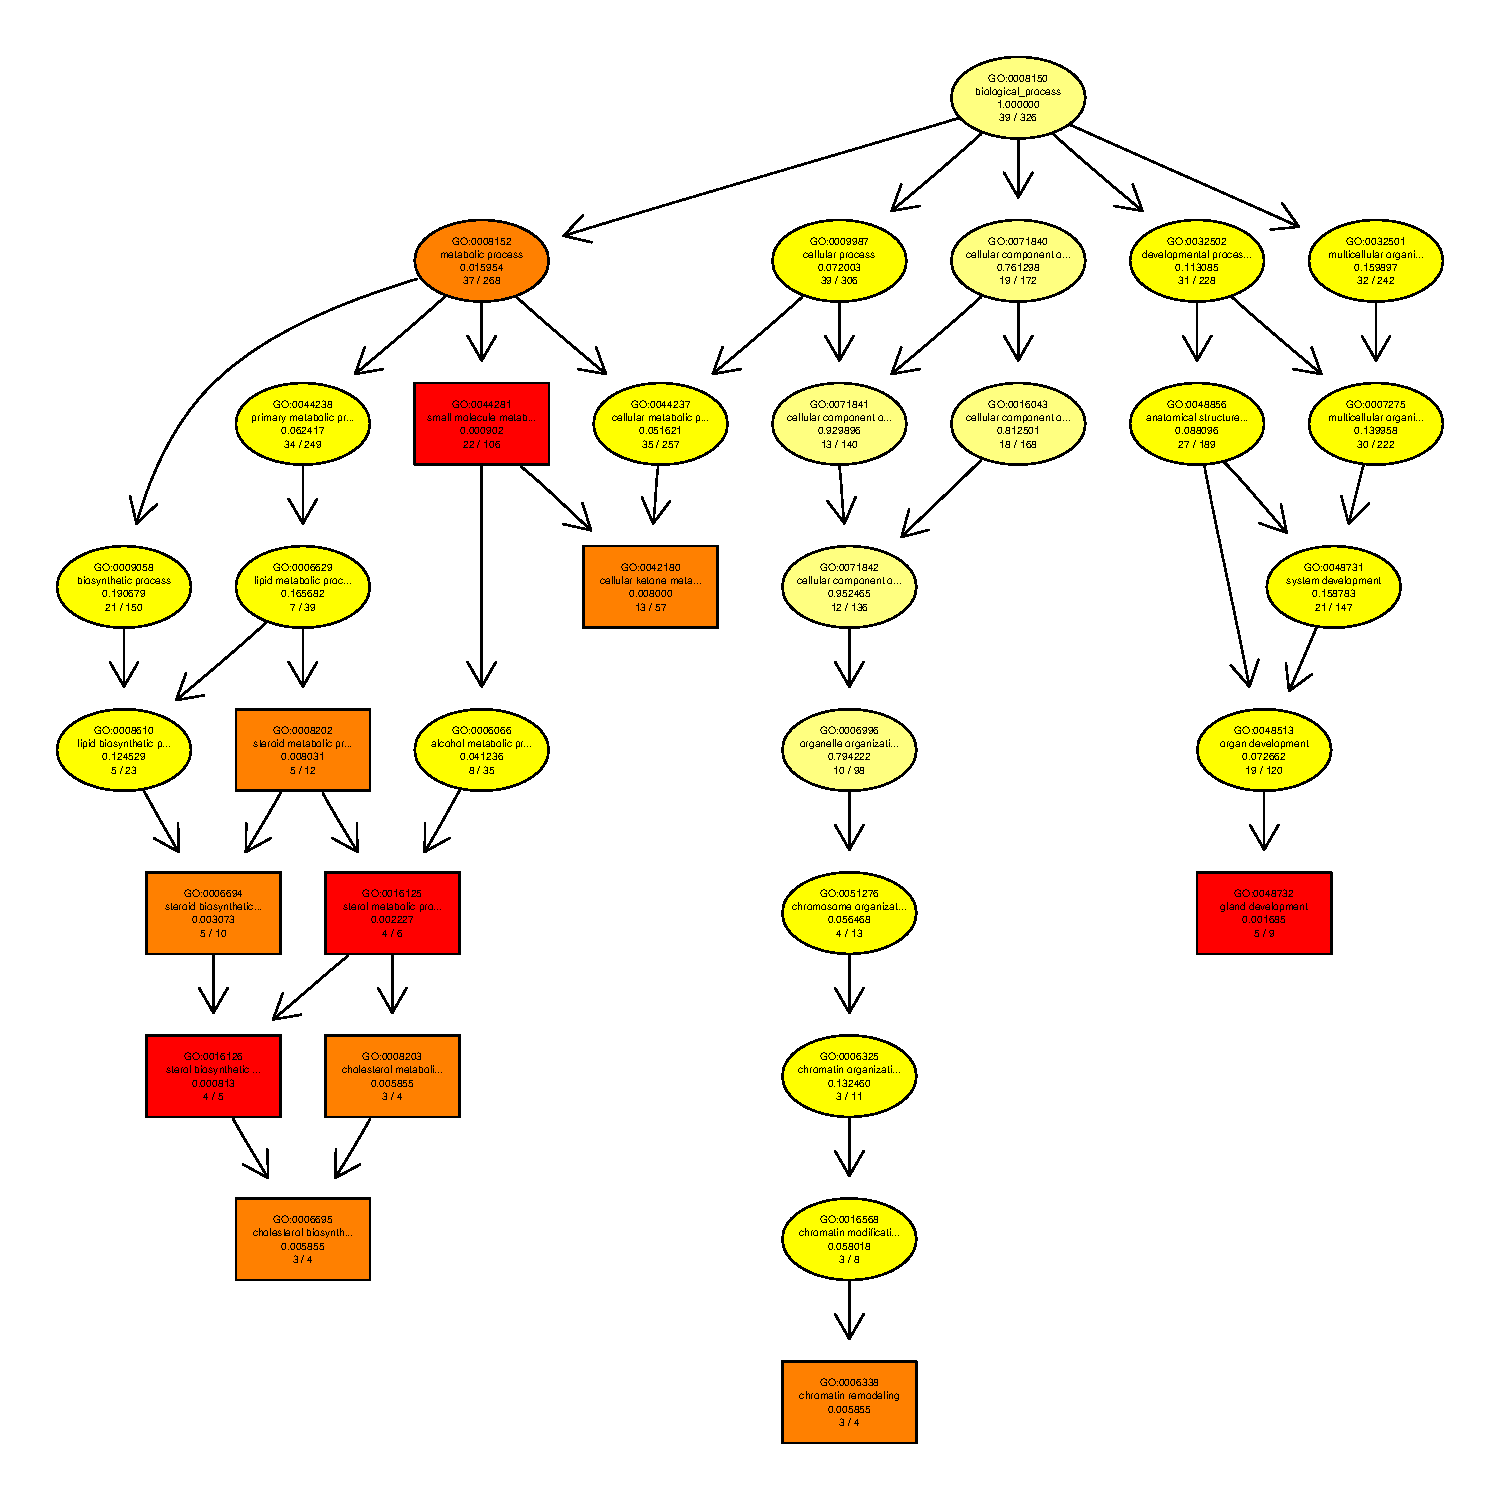
\includegraphics{../figures/tGO_EEL_EXP_BP_classic_10_all}
%   \caption[GO biological process graph for enriched terms in
%   differentially expressed (DE) genes between worm-origin]{GO
%     biological process graph for enriched terms in differentially
%     expressed (DE) genes between worm-origin. Subgraph of the
%     GO-ontology biological process category induced by the top 10
%     terms identified as enriched in DE genes between worms from Asia
%     and Europe. Boxes indicate the 10 most significant terms. Box
%     colour represents the relative significance, ranging from dark red
%     (most significant) to light yellow (least significant). In each
%     node the category-identifier, a (eventually truncated) description
%     of the term, the significance for enrichment and the number of DE
%     / total number of annotated genes is given. Black arrows indicate
%     an ``is-a'' relationship.}{1.3}
% \end{sidewaysfigure}

% \newpage
% \clearpage

% \begin{sidewaysfigure}
%   \centering
%   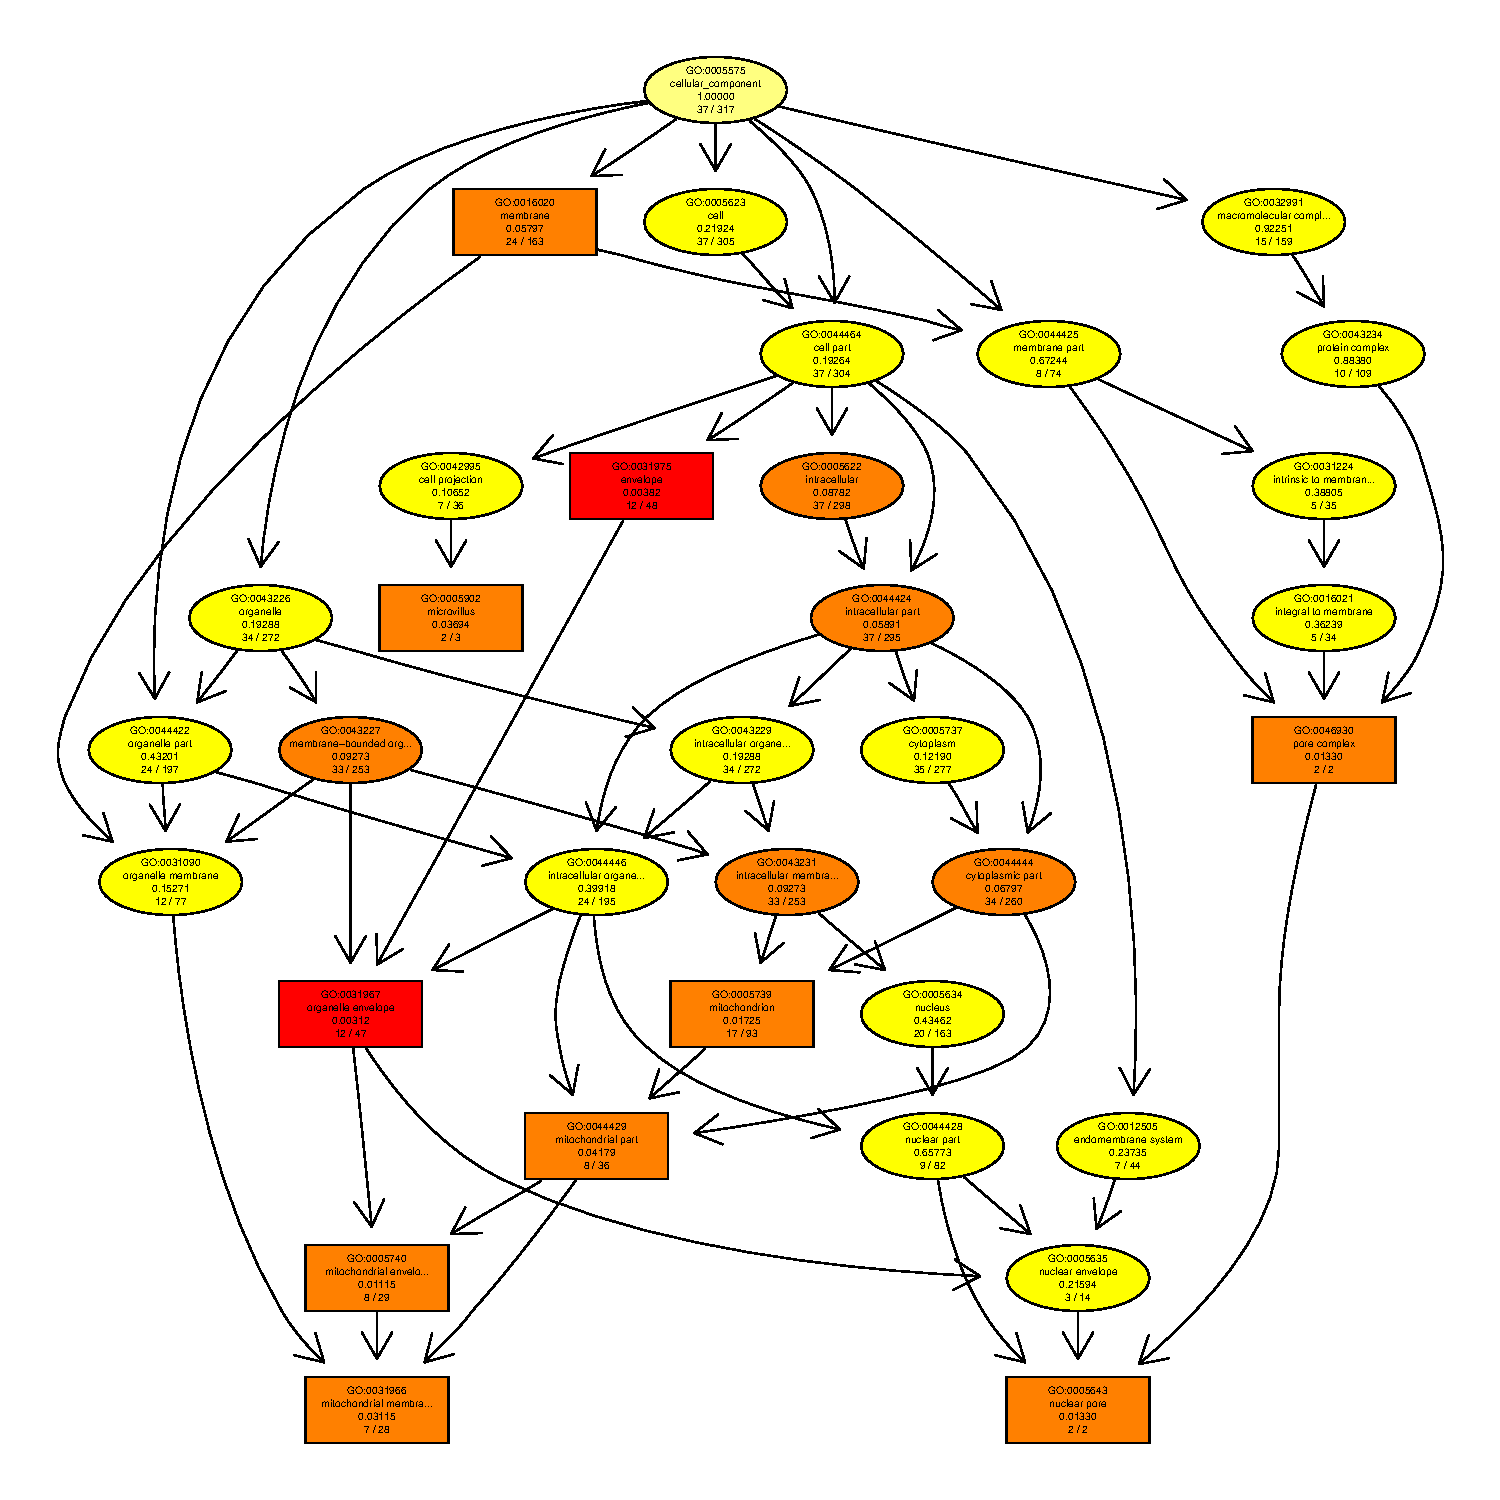
\includegraphics{../figures/tGO_EEL_EXP_CC_classic_10_all}
%   \caption[GO cellular compartment graph for enriched terms in DE
%   genes between worm-origin]{GO cellular compartment graph for
%     enriched terms in DE genes between worm-origin. Subgraph of the
%     GO-ontology cellular compartment category induced by the top 10
%     terms identified as enriched in DE genes between worms from Asia
%     and Europe. Boxes indicate the 10 most significant terms. Box
%     colour represents the relative significance, ranging from dark red
%     (most significant) to light yellow (least significant). In each
%     node the category-identifier, a (eventually truncated) description
%     of the term, the significance for enrichment and the number of DE
%     / total number of annotated genes is given. Black arrows indicate
%     an ``is-a'' relationship.}{1.3}
% \end{sidewaysfigure}

% \newpage
% \clearpage

% \begin{sidewaysfigure}
%   \centering
%   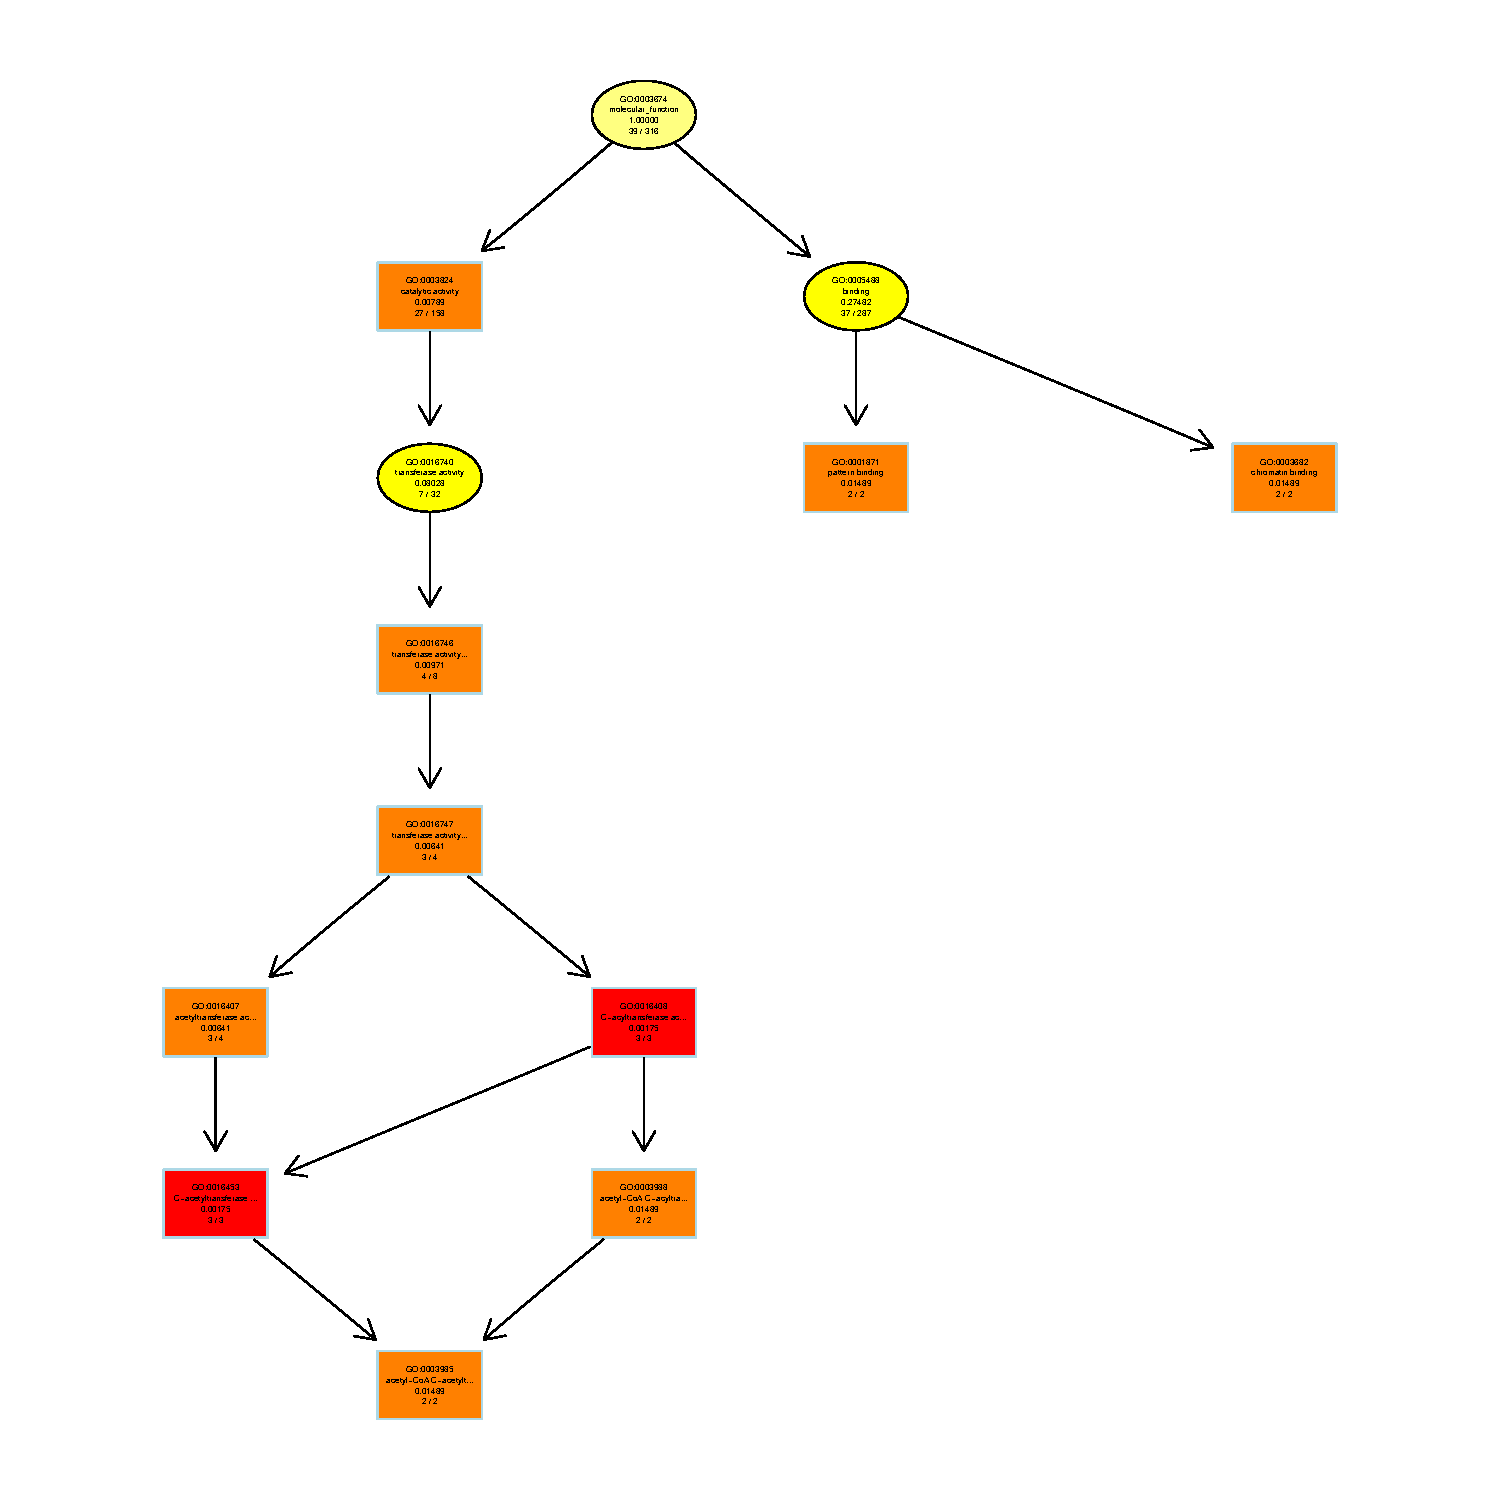
\includegraphics[keepaspectratio=TRUE]{../figures/tGO_EEL_EXP_MF_classic_10_all}
%   \caption[GO molecular function graph for enriched terms in
%   pyrosequencing-DE genes between worm-origin]{GO molecular function
%     graph for enriched terms in DE genes between worm-origin. Subgraph
%     of the GO-ontology molecular function category induced by the top
%     10 terms identified as enriched in DE genes between worms from
%     Asia and Europe. Boxes indicate the 10 most significant terms. Box
%     colour represents the relative significance, ranging from dark red
%     (most significant) to light yellow (least significant). In each
%     node the category-identifier, a (eventually truncated) description
%     of the term, the significance for enrichment and the number of DE
%     / total number of annotated gene is given. Black arrows indicate
%     an ``is-a'' relationship.}{0.9}
% \end{sidewaysfigure}

% \newpage
% \clearpage

% \begin{sidewaysfigure}
%   \centering
%   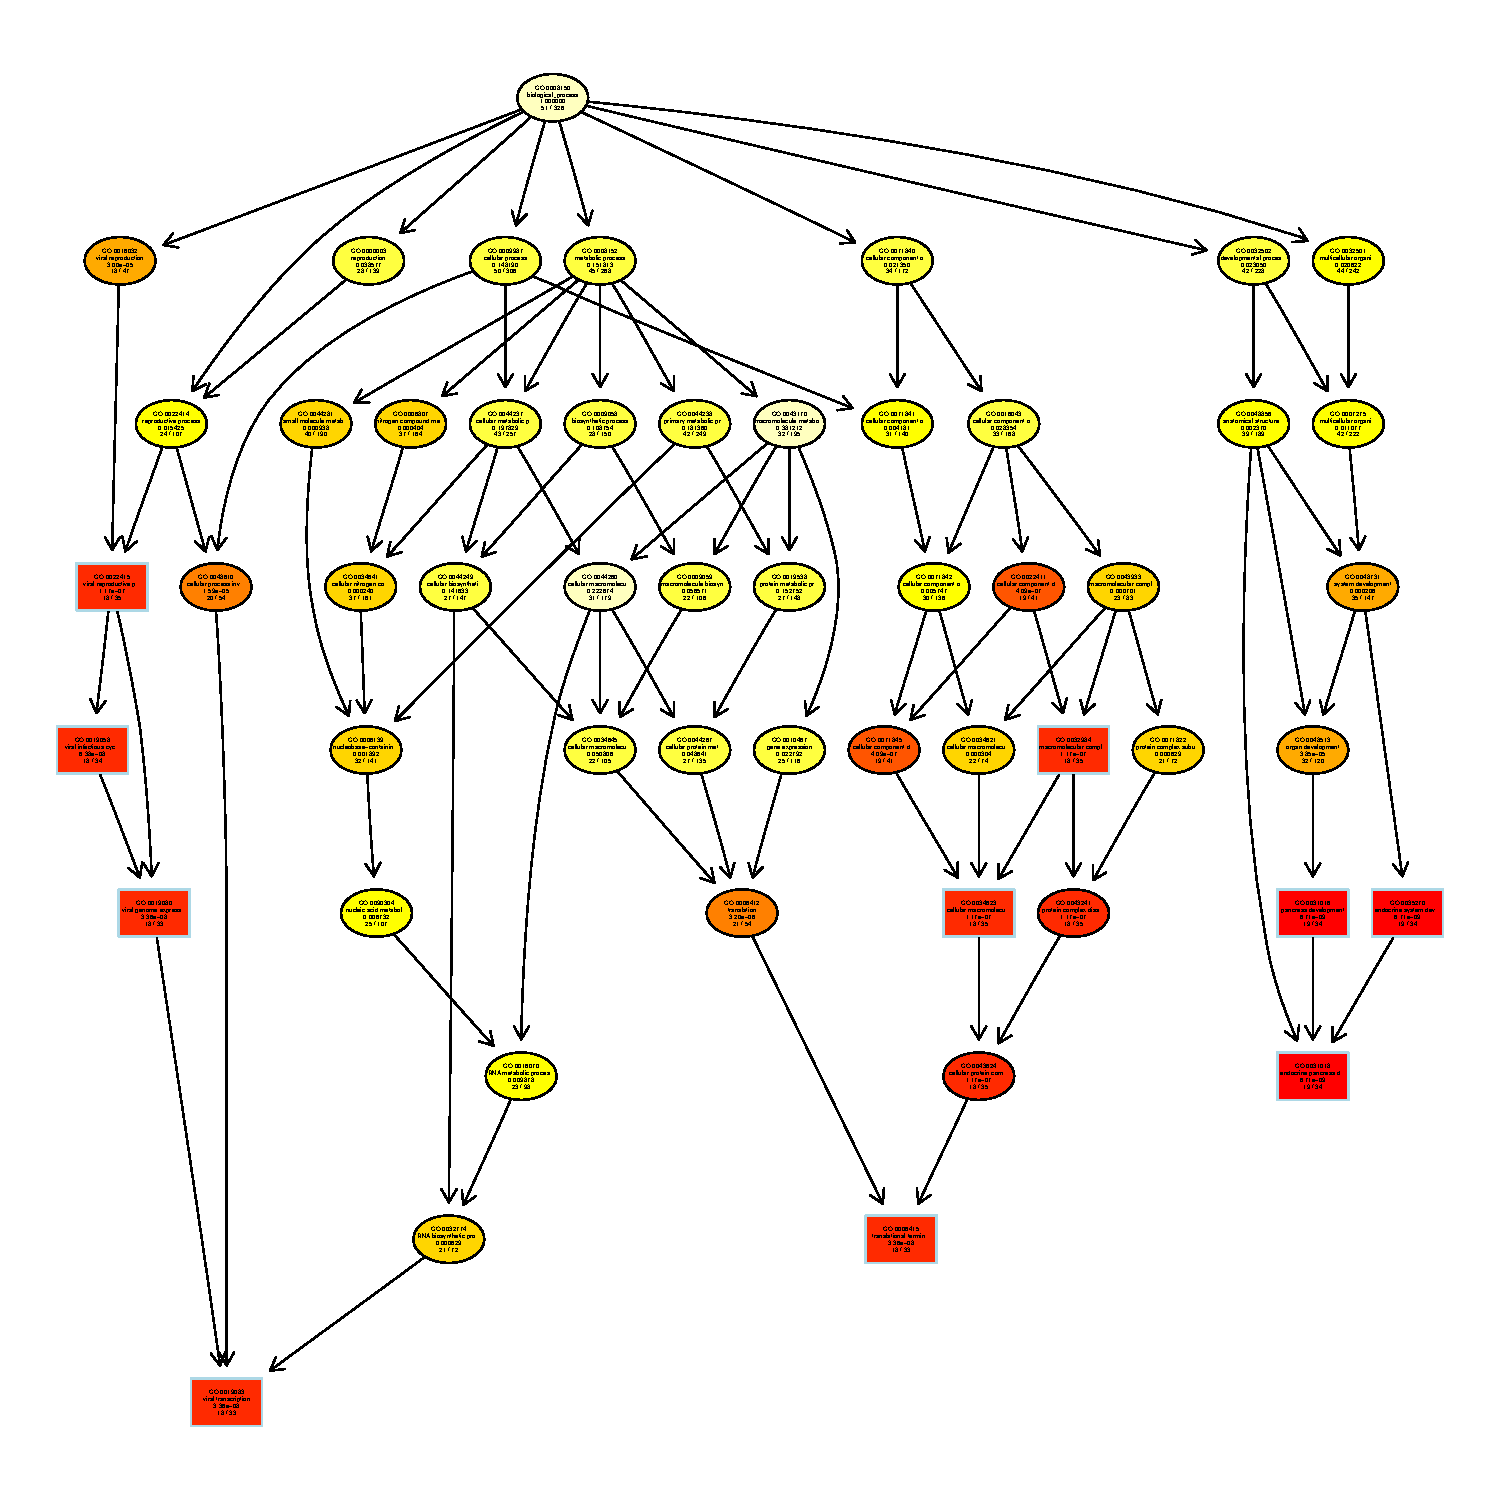
\includegraphics{../figures/tGO_SEX_EXP_BP_classic_10_all}
%   \caption[GO biological process graph for enriched terms in DE genes
%   between worm-sex]{GO biological process graph for enriched terms in
%     DE genes between worm-sex. Subgraph of the GO-ontology cellular
%     compartment category induced by the top 10 terms identified as
%     enriched in DE genes between female and male worms. Boxes indicate
%     the 10 most significant terms. Box colour represents the relative
%     significance, ranging from dark red (most significant) to light
%     yellow (least significant). In each node the category-identifier,
%     a (eventually truncated) description of the term, the significance
%     for enrichment and the number of DE / total number of annotated
%     genes is given. Black arrows indicate an ``is-a''
%     relationship.}{1.3}
% \end{sidewaysfigure}

% \newpage
% \clearpage

% \begin{sidewaysfigure}
%   \centering
%   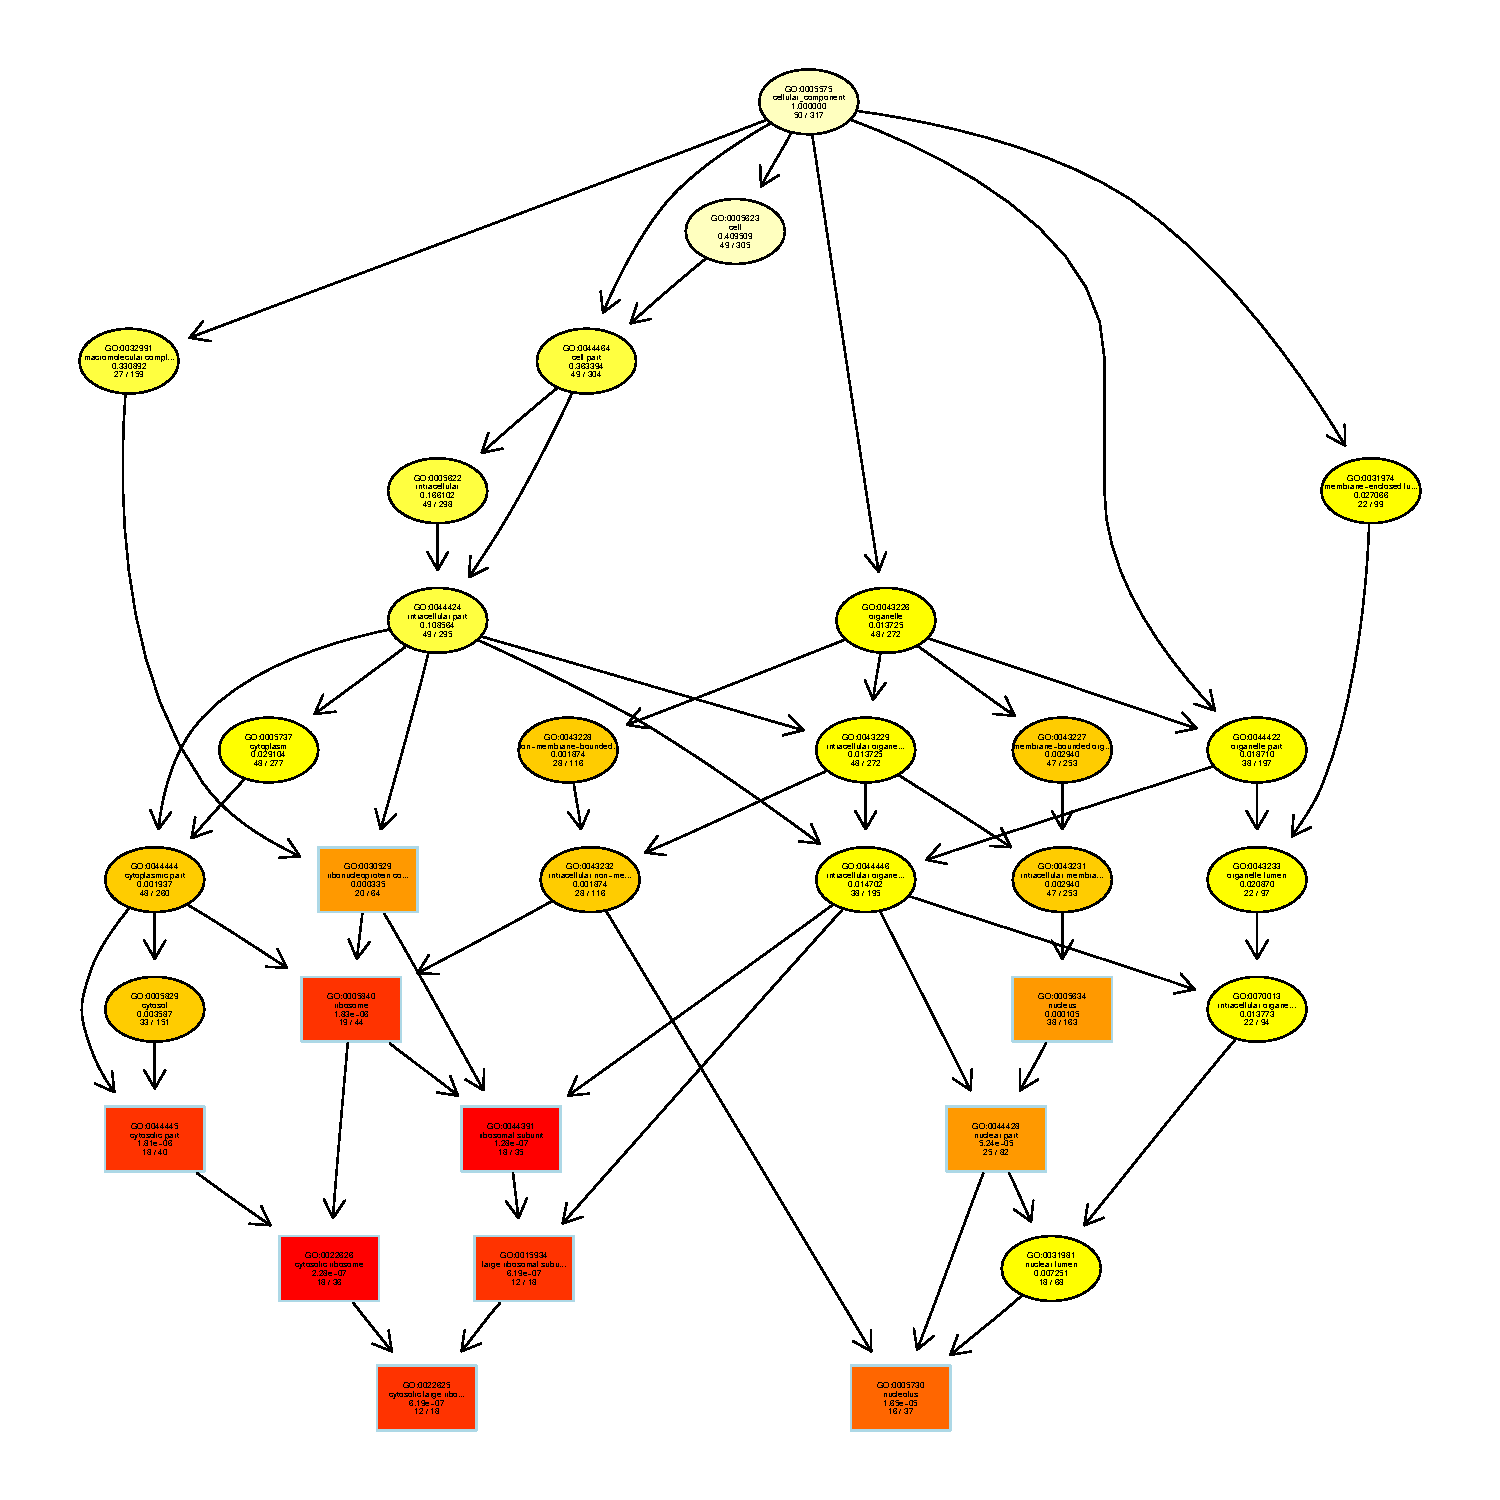
\includegraphics{../figures/tGO_SEX_EXP_CC_classic_10_all}
%   \caption[GO cellular compartment graph for enriched terms in
%   pyrosequencing-DE genes between worm-sex]{GO cellular compartment
%     graph for enriched terms in DE genes between worm-sex. Subgraph of
%     the GO-ontology cellular compartment category induced by the top
%     10 terms identified as enriched in DE genes between female and
%     male worms. Boxes indicate the 10 most significant terms. Box
%     colour represents the relative significance, ranging from dark red
%     (most significant) to light yellow (least significant). In each
%     node the category-identifier, a (eventually truncated) description
%     of the term, the significance for enrichment and the number of DE
%     / total number of annotated genes is given. Black arrows indicate
%     an ``is-a'' relationship.}{1.3}
% \end{sidewaysfigure}

% \newpage
% \clearpage

% \begin{sidewaysfigure}
%   \centering
%   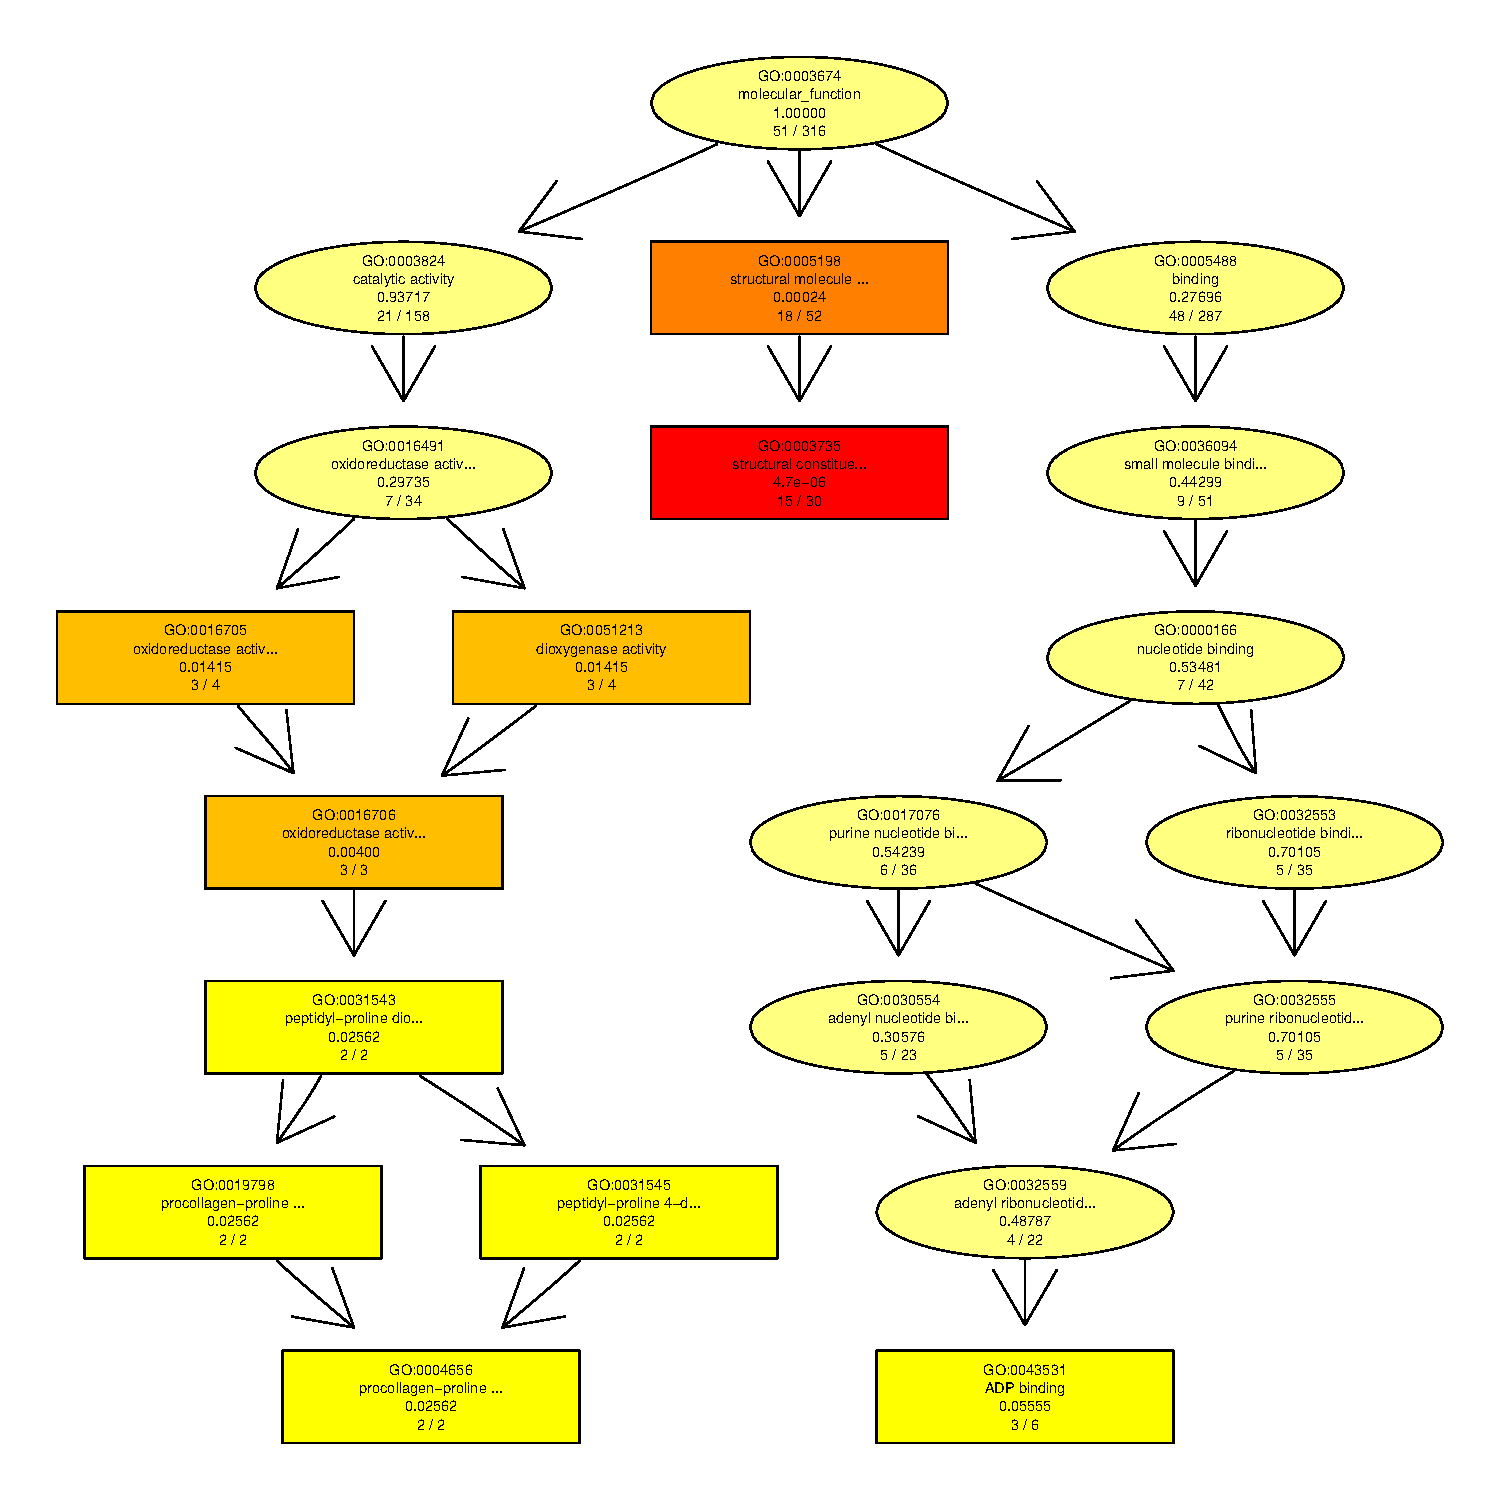
\includegraphics{../figures/tGO_SEX_EXP_MF_classic_10_all}
%   \caption[GO molecular function graph for enriched terms in DE genes
%   between worm-sex]{GO molecular function graph for enriched terms in
%     DE genes between worm-sex. Subgraph of the GO-ontology cellular
%     compartment category induced by the top 10 terms identified as
%     enriched in DE genes between female and male worms. Boxes indicate
%     the 10 most significant terms. Box colour represents the relative
%     significance, ranging from dark red (most significant) to light
%     yellow (least significant). In each node the category-identifier,
%     a (eventually truncated) description of the term, the significance
%     for enrichment and the number of DE / total number of annotated
%     genes is given. Black arrows indicate an ``is-a''
%     relationship.}{1.1}
% \end{sidewaysfigure}

% \newpage
% \clearpage


\section{The transcriptome of \textit{A.crassus}: Evaluating a method of
  combining assemblies}



\subsection{Overview}
\label{sec:overview}

The pre-processed \textit{A. crassus} data-set consisting of
100491819 bases in 353055 reads (58617
generated using ``FLX-chemistry'', 294438 using
``Titanium-chemistry'') was assembled following an approach proposed
by \cite{pmid20950480}: two assemblies were generated, one using
Newbler v2.6 \cite{pmid16056220}, the other using Mira v3.2.1
\cite{miraEST}. The resulting assemblies (referred to as first-order
assemblies) were merged with Cap3 \cite{Cap3_Huang} into a combined
assembly (referred to as second-order assembly).


\subsection{The Newbler first-order assembly}
\label{sec:new-fist}




During transcriptome assembly (with options -cdna -urt) Newbler can
split individual reads spanning the breakpoints of alternate isoforms,
to assemble e.g. the first portion of the reads in one contig and the
second portion in two different contigs. Subsequently, multiple so
called isotigs are constructed and reported, one for each putative
transcript variant. While this approach could be helpful for the
detection of alternate isoforms, it also produces short contigs
(especially at error-prone edges of high-coverage transcripts) when
the building of isotigs fails. The read status report and the assembly
output in ace format the program provides include short contigs only
used during the assembly process, but not reported in the contigs file
used in transcriptome-assembly projects (454Isotigs.fna). Therefore to
get all reads not included in contigs (i.e. a consistent definition of
``singleton'') it was necessary to add all reads appearing only in
contigs not reported in the fasta file to the reported singletons. The
number of singletons increased in this step from the
26211 reported to
109052. We later also address the usefulness of
Newbler's report vs. the expanded singleton-category, but for the
meantime we define singletons as all reads not present in contigs
reported from a given assembly.

\newpage
  

\begin{figure}[H]
  \centering
  
\includegraphics{Supporting_information-008}

\caption{A histogram of the number of contigs/isotigs that individual
  reads are split into by the Newbler assembly.}
  \label{fig:newdist}
\end{figure}

While, the splitting of reads in the Newbler assembly can give useful
information on possible isoforms, the number of contigs Newbler split
one read into (in some cases more than 100 contigs) seems inflated
(see additional figure \ref{fig:newdist}). This emphasises the need
for further processing of the contigs. The maximum number of read
splits in a contig and its usefulness in estimating contig quality
will be discussed later in greater detail.

\subsection{The Mira assembly and the second-order assembly}
\label{sec:assembly-sec}

The Mira assembly (with options --job=denovo,est,accurate,454)
provided a second estimate of the transcriptome. In this assembly
individual reads were not split. The number of reads not used in the
Mira assembly was 65368.

To combine the two assemblies Cap3 was used with default parameters
and the quality information from first-order assemblies was
included. Below, we explore how information from both estimates of the
transcriptome were integrated into the final second-order assembly.

% latex table generated in R 2.16.0 by xtable 1.7-0 package
% Thu Jun 21 10:52:41 2012
\begin{table}[ht]
\begin{center}
\begin{tabular}{rlll}
  \hline
 & Newbler & Mira & Second-order(MN) \\ 
  \hline
Max length & 6300 & 6352 & 6377 \\ 
  Number of contigs & 15934 & 22596 & 14064 \\ 
  Number of Bases &  8085922 & 12010349 &  8139143 \\ 
  N50 & 579 & 579 & 662 \\ 
  Number of congtigs in N50 & 4301 & 6749 & 3899 \\ 
  non ATGC bases &   375 & 29962 &  5245 \\ 
  Mean length & 508 & 532 & 579 \\ 
  Number of singletons & 26211/109052 & 65368 & 23175/47669 \\ 
  Span of singletons & 7022901/31670649 & 17833358 & 6108621/13291587 \\ 
   \hline
\end{tabular}
\caption[Basic statistics for the first-order assemblies and the second-order assembly]{Basic statistics for the first-order assemblies and the second-order assembly (for which only the most reliable category of contigs is shown. For Newbler the number of singletons is given as defined above as ``unused reads'' and as reported. Singletons for the second-order assembly are the intersection of these with the Mira singletons.}
\label{tab:pc}
\end{center}
\end{table}
Additional table \ref{tab:pc} gives summary statistics of the different
assemblies. Mira clearly produced the biggest assembly, both in terms
of number of contigs and bases). The second-order assembly is slightly
smaller than the Newbler assembly.  The second-order assembly had on
average longer contigs than both first-order assemblies and a higher
weighted median contig size (N50).



\newpage
\subsection{Data categories in the second-order assembly}
\label{sec:data-categ-second}

Three main categories of assembled sequence data can be distinguished
in the second-order assembly, each one with different reliability and
utility in downstream applications:

The first category of data obtained are the singletons of the final
second-order assembly. It comprises raw sequencing reads that neither
of the first-order assemblers used. It is therefore the intersecion of
the Newbler singletons (as defined in \ref{sec:new-fist}) and the Mira
singletons. 47669 reads fell in this category. A
second category of sequence is the first-order contigs that were not
assembled in the second-order assembly (the singletons in the Cap3
assembly; M\_1 and N\_1 in additional table
\ref{tab:categ}). Second-order contigs in which first-order contigs
from only one assembler are combined (M\_n and N\_n in additional
table \ref{tab:categ}) were also included in this category. We
consider sequences in this category as only moderately reliable, as
they are supported by only one assembly algorithm. The category of
contigs considered the most reliable contains all second-order contigs
with contribution from both first-order assemblies (MN in additional
table \ref{tab:categ}). For this last, most reliable (MN) category,
reads contained in the assembly can be categorised depending on
whether they entered the assembly via both or only via one first-order
assembly.

% latex table generated in R 2.16.0 by xtable 1.7-0 package
% Thu Jun 21 10:52:47 2012
\begin{table}[ht]
\begin{center}
\begin{tabular}{p{2.5cm}llcll}
  \hline
 & M\_1 & M\_n & MN & N\_n & N\_1 \\ 
  \hline
Second order contigs &   & 164 & 13887 & 13 &   \\ 
  First order contigs & 2347 & 897 & mira=19352/Newbler=14410 & 40 & 1484 \\ 
  reads & 42172 & 21153 & one=269868/both=193308 & 1538 & 13100 \\ 
   \hline
\end{tabular}
\caption[Number of reads, first-order contigs and second-order contigs for different categories of contigs]{Number of reads, first-order contigs and second-order contigs for different categories of contigs (M\_1 and N\_1 = first-order contigs not assembled in second-order assembly, from mira and newbler respectively; M\_n and N\_n =  assembled in second-order contigs only with contigs from the same first-order assembly; MN = assembled in second-order contigs with first order contigs from both first order assemblies}
\label{tab:categ}
\end{center}
\end{table}
\newpage

\begin{figure}[H]
  \centering
  

\includegraphics{Supporting_information-014}

\caption{Classification of reads by the route they followed into the
  final combined assembly (MN category only))}
\label{fig:venncat}
\end{figure}

Additional figure \ref{fig:venncat} gives a more detailed view of the fate of the
reads split by Newbler during first-order assembly. Interestingly most
reads split by Newbler ended up in the high-quality category of the
second order assembly.

\subsection{Contribution of first-order assemblies to second-order contigs}
\label{sec:contr-firs-order}

  

Examining the contributions of contigs from each of the assemblies to
one second-order contig in additional figure \ref{fig:rcp}a it becomes
clear that the Mira assembly had many redundant contigs. The reads
contributing to these were assembled into the same contig by Newbler
and finally also into one second-order contig by Cap3.


\begin{figure}[H]
  \centering

\includegraphics{Supporting_information-018}


\caption[Contig and read contribution to second-order contigs.]{
  Contig and read contribution to second-order contigs. (a) Number of
  first-order contigs from both first-order assemblies for each second
  order contig. (b) Number of reads through Newbler and Mira for each
  second-order contig.}
\label{fig:rcp}
  
\end{figure}


A different picture emerges from examination of the contribution of
reads through each of the first-order assemblies (additional figure
\ref{fig:rcp}b).  Here, for most second-order contigs, many more reads
are contributed through Newbler contigs. This is because Newbler has
more reads summed over all contigs, due to the duplication resulting
from splitting of reads.

\newpage

\subsection{Evaluation of the assemblies}
\label{sec:eval-three-assembl}


To further compare assemblies (Mira or Newbler first-order assemblies
including or excluding their singletons) and the second-order assembly
(including different contig categories and singletons) we evaluated
the number of bases or proteins their contigs and singletons
(partially) cover in the related model nematodes,
\textit{Caenorhabditis elegans} and \textit{Brugia malayi}. For this
purpose we used BLAST (blastx E-value cut-off 1e-5) and a custom perl
script provided by S. Kumar (mask\_blast.pl available from
github.com/sujaikumar/assemblage).

In addition, the span of an assembly can give an indication of
redundancy or artificially assembled data. If span increases without
reference coverage, the dataset is likely to contain more redundant or
artificial information, and a more parsimonious assembly should be
preferred. The coverage for the two reference species was plotted
against the size of the assembly dataset to estimate the completeness
conditional on the size of the assembly (additional figures
\ref{fig:basecov}, \ref{fig:protcov}, \ref{fig:prot80cov}).

From the assemblies excluding singletons (in the lower left corners of
additional figures \ref{fig:basecov}, \ref{fig:protcov} and
\ref{fig:prot80cov}; with lower size and database coverage) the highly
reliable second order assembly contigs produced the highest per-base
coverage in both reference species, with the Newbler assembly second
and Mira producing the lowest reference coverage. When the contigs
considered lower quality (i.e. supported by only one assembler) were
added to the second-order assembly, reference coverage increased
moderately.

A comparison of the addition of only Newbler's reported singletons and
the addition of all singletons to the Newbler assembly showed that the
reported singletons increased reference coverage to the same extent as
all singletons, while the non-reported singletons only increased the
size of the assembly. It can be concluded that the latter contain very
little additional biological information and are likely to include
only error-prone or variant reads.

The second-order assembly including the intersection of first-order
singletons had similar reference coverage metrics to the Newbler
assembly, but was larger in size. Adding the less reliable set of
one-assembler supported second-order contigs the assembly covered the
most bases in both references. When the intersection of the Newbler
``reported singletons'' and Mira singletons was added a parsimonious
assembly with high reference coverage (termed fullest assembly; and
labeled FU in additional figures \ref{fig:basecov}, \ref{fig:protcov}
and \ref{fig:prot80cov}) was obtained.

\begin{sidewaysfigure}

\includegraphics{Supporting_information-020}
\caption[Span and reference transcriptome coverage (in bases)]{Span
  and reference transcriptome coverage (in bases) for different
  assemblies and assembly-combinations. M = Mira; N = Newbler; $M+S$ =
  Mira + singletons; $N+S$ = Newbler plus singletons; $N+Sr$ = Newbler
  plus singletons reported in readstatus.txt; MN = second-order
  contigs supported by both first-order; $MN+N\_x$ = second-order MN
  plus contigs only supported by Newbler ($N\_x$ = $N\_n$ and $N\_1$);
  $MN+M\_x$ = same for Mira-first-order-contigs; $MN+M\_x+S$ and
  $MN+N\_x+S$ same with singletons; FU = second-order contigs
  supported by both or one assembler plus the intersection of Newbler
  reported singletons and Mira-singletons = the basis for the
  ``fullest assembly'' used in later analyses.}
\label{fig:basecov}
\end{sidewaysfigure}


\begin{sidewaysfigure}

\includegraphics{Supporting_information-021}
\caption[Span and reference transcriptome coverage in percent of
proteins hit]{Span and reference transcriptome coverage in percent of
  proteins hit for different assemblies and assembly-combinations. For
  category abrevations see additional figure \ref{fig:basecov}.}
\label{fig:protcov}
\end{sidewaysfigure}

\begin{sidewaysfigure}

\includegraphics{Supporting_information-022}
\caption[Span and reference transcriptome coverage in percent of
proteins coverd to at least 80\% of their length]{Span and reference
  transcriptome coverage in percent of proteins coverd to at least
  80\% of their length for different assemblies and assembly
  combinations. For category abrevations see additional figure
  \ref{fig:basecov}.}
\label{fig:prot80cov}
\end{sidewaysfigure}

When database proteins covered for at least 80\% of their length are
considered (additonal figure \ref{fig:prot80cov}) the second-order
assembly was superior: Both ex- and in-cluding singletons the
second-order assembly outperformed the first-order
assemblies. Moderate gains in reference coverage were made again for
the addition of dubious single assembler supported second-order
contigs. 

Given this evaluation we defined the ``minimal adequate assembly'' as
the subset of contigs of the second-order assembly supported by both
assemblers (labeled MN above). Given the performance of the singletons
Newbler reported, we defined the ``fullest assembly'' as all
second-order contigs (including those supported by only one assembler)
plus the intersection of reported Newbler singletons and Mira
singletons.

The proportion of proteins covered in \textit{C. elegans} by
\textit{B. malayi} coding sequences was with
26.85\% simimlar to our estimate for
the fullest (FU) assembly. The proportion of bases
(25.46\%) and of proteins coverd to
at least 80\% of their length
(14.67\%) was however higher for
the coding sequences from \textit{B. malayi}.

\subsection{Measurments on second-order assembly}

Based on the tracking of reads through the assembly process, we
calculated the following statistics for each contig in the
second-order assembly.

\begin{itemize}
\item number of Mira and Newbler first-order contigs
\item number of reads in each contributing Mira contig and Newbler
  contig
\item number of reads split by Newbler in first-order assembly
\item number of read-split events in the first-order assembly (the sum
  of reads multiplied by number of contigs a read has been split into)
\item maximal number of first-order contigs a read in the contig has
  been split into during Newbler assembly
\item the number of reads same-read-paires from the Newbler and Mira
  first order-assembly merged in a second order contig
\item cluster-id of the contig: the cluster to which the contig
  belongs (contigs ``connected'' by sharing reads are placed in one
  cluster; similar to the graph clustering reported in
  \cite{pmid21138572}).
\item number of other second-order contigs containing the same read
  i.e. the size of the cluster
\end{itemize}



\subsubsection{Contig coverage}



As well defined coverage-information was not readily avaiable from the
output of this combined assembly aproach (although we followed
individual reads through the process) we inferred coverage by mapping
the reads used for assembly against the fullest assembly using ssaha2
\cite{pmid11591649} with parameters (-kmer 13 -skip 3 -seeds 6 -score
100 -cmatch 10 -ckmer 6 -output sam -best 1). This read mapping was
summarised by:

\begin{itemize}
\item mean per base coverage
\item mean unique per base coverage
\end{itemize}

The ratio of mean per base coverage and unique per base coverage (the
standard for assessing coverage) can be used to assess the redundancy
of a contig.

\subsubsection{Example use of the contig-measurements}

Based on these measurements the generation of a given contig by the
assembly process can be reconstructed. Additional table
\ref{tab:ex-me} gives an excerpt of the contig-measurements reported
in additional file A.crassus\_transcriptome\_contig\_data.csv. The
example contigs are all from large contig clusters (cluster.size),
where interpretation of the assembly history is more complex:

% latex table generated in R 2.16.0 by xtable 1.7-0 package
% Thu Jun 21 10:56:58 2012
\begin{table}[ht]
\begin{center}
\begin{tabular}{rllll}
  \hline
 & Contig1047 & Contig10719 & Contig104 & Contig13672 \\ 
  \hline
reads\_through\_Newbler &   16 & 1351 &    0 &   14 \\ 
  reads\_through\_Mira &  26 & 651 & 135 &   0 \\ 
  Newbler\_contigs & 1 & 5 & 0 & 2 \\ 
  Mira\_contigs & 1 & 9 & 4 & 0 \\ 
  category & MN & MN & M\_n & N\_n \\ 
  num.new.split &    8 & 1314 &    0 &    0 \\ 
  sum.new.split &   16 & 2628 &    0 &    0 \\ 
  max.new.split & 2 & 2 & 0 & 0 \\ 
  num.SndO.pair &  13 & 644 &   0 &   0 \\ 
  cluster.id & CL62 & CL6 & CL176 & CL235 \\ 
  cluster.size & 24 & 18 &  5 &  5 \\ 
  coverage &   4.200342 & 267.495458 &  41.003369 &   2.920755 \\ 
  uniq\_coverage & 4.248960 & 7.425507 & 2.568000 & 1.196078 \\ 
   \hline
\end{tabular}
\caption{example table for assembly-measurements on contigs (as given in
                         A.crassus\_transcriptome\_contig\_data.csv)}
\label{tab:ex-me}
\end{center}
\end{table}
\textbf{Contig1047} is from the well trusted MN category of
contigs. It consists of only one contig from each first-order assembly
(newbler\_contigs and mira\_contigs), each containing a set of reads
of moderate size: 16 from Newbler (reads\_through\_newbler), and 26
from Mira (reads\_through\_mira). 8 of the 16 reads Newbler used were
also assembled to a differnt Newbler contig (num.new.split). That each
of the 8 reads only appeared in one other Newbler contig is evident as
the number of split events is 16 (sum.new.split) and the maximal
number of splits for one read is 2 (max.new.split). 13 (num.SndO.pair)
same-read-pairs from the two different first-order assemblies were
merged in this second-order contig, leaving 3 (16-13) reads in Newbler
contigs and 13 (26-13) reads in Mira contigs, which all could
potentially have ended up in other contigs. The contig is in a cluster
(CL62), which contains 24 contigs (cluster.size). The complete graph
structure linking these 24 contigs cannot be reconstructed from this
contig summary data. The summary data makes clear the sources of links
for cluster-affiliation: In the case of Contig1047 from 3 and 13
unlinked read-paires from both first-order assemblies and 8 split
reads from Newbler first-order contigs.

A comprehensive interpretation of the other example contigs depicted
is left to the reader. It should just be remarked, that in case of
one-assembler supported contigs, all reads in that contig could
potentially be represented in other contigs, making average
cluster-size in these contigs bigger than in MN category.\\

Interesting measurements calculated for each contig include the
cluster membership and cluster size. Such clusters represent close
paralogs, duplicated genes, isoforms from alternative splicing or
allelic variants. These measurements can be used in later analysis to
e.g. reevaluate the likelihood of misassembly in a given set of
biologically relevant contigs. All gene sets discussed in the main
text were, as a matter of routine, controlled for unusual patterns in
the contig meta-data.

\subsection{Finalising the fullest assembly set}
\label{sec:final-full-assembly}

In order to minimize the amount of sequence with artificially inferred
isoform breakpoints we used the unique mapping information described
above to detect contigs and singletons not supported by any
independent raw data (reads). Additional table \ref{tab:cov.ex} gives
a summary of these unsupported data by contig category. For all
downstream analyses we removed all the MN-category contigs and the
contigs (and singletons) from other categories having no unique
coverage.

% latex table generated in R 2.16.0 by xtable 1.7-0 package
% Thu Jun 21 10:56:58 2012
\begin{table}[ht]
\begin{center}
\begin{tabular}{rrrrrrr}
  \hline
 & singletons & M\_1 & M\_n & MN & N\_1 & N\_n \\ 
  \hline
coverage == 0 & 546 &  34 &   2 &  36 & 158 &   0 \\ 
  unique coverage == 0 & 584 &  48 &   2 &  42 & 210 &   3 \\ 
   \hline
\end{tabular}
\caption{number of contigs with a coverage and unique-coverage of zero, inferred from mapping of raw reads, listed by contig-category}
\label{tab:cov.ex}
\end{center}
\end{table}
The remaining 40,187 tentative unique genes (TUGs), define the
``fullest assembly''. The MN-category of contigs form the high
credibility assembly (highCA) and the M\_n, N\_n, M\_1, N\_1 and
Newbler's reported singletons are the additional low credibility
assembly (lowCA).


%%%%%%%%%%%%%%%%%%%%%%%%%%%%%%%%%%%%%%%%%%%%%%%%%%%%%%%%%%%%%
%%                  The Bibliography                       %%
%%                                                         %%              
%%  Bmc_article.bst  will be used to                       %%
%%  create a .BBL file for submission, which includes      %%
%%  XML structured for BMC.                                %%
%%                                                         %%
%%                                                         %%
%%  Note that the displayed Bibliography will not          %% 
%%  necessarily be rendered by Latex exactly as specified  %%
%%  in the online Instructions for Authors.                %% 
%%                                                         %%
%%%%%%%%%%%%%%%%%%%%%%%%%%%%%%%%%%%%%%%%%%%%%%%%%%%%%%%%%%%%%


\bibliographystyle{/home/ele/bibtex/bmc_article.bst} % Style BST file
\newpage
\bibliography{/home/ele/bibtex/master.bib} % Bibliography file (usually '*.bib' )


\end{document}
